%% =============================
% * <romulolins2001@gmail.com> 2018-08-09T22:36:34.296Z:
%
% ^.
%%      IMPORTANTE
%% ESTE ARQUIVO DEVE ESTAR SALVO COMO
%%      UTF - 8
%% =============================

% ----------------------------------------------------------
% Este arquivo é o arquivo mestre
% Relatorio_TCC_Mestrado_Base_VERSÃO_SUBVERSÃO_FHZ
% Ele contém as classes, formatações e pacotes usadas
% Contém as informações bases para capas e elementos não textuais
% Contém a chamada dos arquivos externos
% ----------------------------------------------------------

%% =====================================
%% The original source files were:
%%
%% coppe.dtx  (with options: `example')
%%
%% This is a sample monograph which illustrates the use of `ufabc' document
%% class and `coppe-unsrt' BibTeX style.
%% =====================================

%% ===================================== ufabcFHZ
%% Esta versão para uso da UFABC gera a classe `ufabcFHZ#.dtx'
%% 		onde # se refere a letra usada para controle das versões
%% As classes `ufabcFHZ#.cls' possuem comentários explicitando os blocos de comandos usados e o histórico das versões.
%%
%% O gerador de referências `abntFHZ#.bst' 
%% 		onde # se refere ao número usado para controle das versões
%%
%% Esta é a versão `ufabcFHZ_LaTeX_Posgrad_v05' - 09.11.2016
%% 		Organizando os arquivos em LaTeX para o trabalho, comandos personalizados e pacotes inseridos
%%
%% ufabcFHZh:
%% Author(s): FHZ - B. Eng. Fernando Henrique G. Zucatelli
%% 			  Prof. Dr. Magno Enrique Mendoza Meza
%% Collaboration(s):
%% 			  B.Eng. Reginaldo Cardoso
%% Translator(s):
%% 			  FHZ & Reginaldo
%% =====================================


% -----------------------------------------
% Classe do documento ufabcFHZh.cls
% -----------------------------------------
% ----------------------------------------- Versão econômica em português
%\documentclass[dsc]{ufabcFHZh}
% ----------------------------------------- Versão final em português
\documentclass[msc, PT, VF]{ufabcFHZh}
% ----------------------------------------- Versão econômica em inglês
%\documentclass[msc, EN]{ufabcFHZh}
% ----------------------------------------- Versão final em inglês
%\documentclass[msc, EN, VF]{ufabcFHZh}
% -----------------------------------------
% ---- Opções da classe:
%%% msc 	- Mestrado  - Dissertação
%%% dscexam	- Doutorado - Exame de Qualificação
%%% dsc 	- Doutorado - Tese
%%% -- // -- // -- Seleção de idiomas, PT é padrão em caso de vazio/omissão
%%% É necessário compilar duas vezes seguidas para atualizar o arquivo após alterar o idioma
%%% (Vazio) - Português
%%% EN - English
%%% -- // -- // -- Versão Final ou Econômica
%%% omissão - versão econômica
%%% VF 		- Versão Final
%%% A impressão da versão final deve conter os elementos pré-textuais apenas nas folhas ímpares (lado direito), exceto a ficha catalográfica que fica no verso da folha de rosto, todavia as páginas em branco devem ser contadas, e os elementos textuais e pós-textuais em ambos os lados\footnote{Guia de nornamlização pós-graduações UFABC \url{http://propg.ufabc.edu.br/wp-content/uploads/guia-normalizacao.pdf}}.
%%% 	De tal forma que a solução mais simples é sempre imprimir frente e verso
% ----

% -----------------------------------------
% Codificação - Comandos personalizados - Seleção de cores nos links - Pacotes
% -----------------------------------------
% ========= Codificação
\usepackage[T1]{fontenc}
%\usepackage[latin1]{inputenc}
\usepackage[utf8]{inputenc}
% =========
\usepackage{pgfplots}
% ========== Novos comandos para escrever nomes pré-formatados
%% =============================
%%      IMPORTANTE
%% ESTE ARQUIVO DEVE ESTAR SALVO COMO
%%      UTF - 8
%% =============================

% ----------------------------------------------------------
% Este capítulo é parte integrante do arquivo mestre
% Relatorio_TCC_Mestrado_Base_VERSÃO_SUBVERSÃO
% ----------------------------------------------------------

%==== Novos comandos para escrever nomes pré-formatados
%---
\newcommand{\ufabcFHZ}
{\textbf{\textit{ufabcFHZh.cls}}}
%---
\newcommand{\abntFHZ}
{\textbf{\textit{abntFHZ5.bst}}}
%---
\newcommand{\Fonte}[1]
{{\footnotesize Fonte: #1.}}
%---
\newcommand{\Oautor}
{O autor}
%---
\newcommand{\matlab}
%{Matlab$^\circledR$}
{Matlab\textsuperscript{\textregistered}}
%---
\newcommand{\simulink}
{Simulink\textsuperscript{\textregistered}}
%---
\newcommand{\matlabsimulink}
{Matlab/Simulink\textsuperscript{\textregistered}}
%---
\newcommand{\arduino}
{Arduino\textsuperscript{\textregistered}}
%---
\newcommand{\arduinomega}
{Arduino\textsuperscript{\textregistered} Mega}

%---
\newcommand{\DINAMA}
{\textit{DINAMA}}
%---
\newcommand{\excel}
{Excel\textsuperscript{\textregistered}}
%---
\newcommand{\projetoDaniel}
{\textit{Projeto Daniel}}
%---
\newcommand{\notimpossiblenow}
{\textit{Not Impossible\textsuperscript{Now}}}
%---
\newcommand{\caltech}
{\textit{Caltech}}
%====

% ----------------------------------------- 
% Formas de uso de condicional ifthenelse / toogle para selecionar cores de links
% -----------------------------------------
% http://alvinalexander.com/blog/post/latex/two-simple-examples-using-latex-ifthen-package
% http://tex.stackexchange.com/questions/5894/latex-conditional-expression
% -----------------------------------------
\usepackage{etoolbox} 		% Permite o uso de \newtoggle para criar desvios de fluxo
\usepackage{pdfpages}
%---
\newtoggle{LinksComCores} 	% Opção para selecionar entre links sem cores ou coloridos
% ===
% -----------------------------------------

% ----------------------------------------------------------
% Fim Arquivo
% \usepackage[alf, abnt-emphasize=bf, abnt-thesis-year=both, abnt-repeated-author-omit=no, abnt-last-names=abnt, abnt-etal-cite=3, abnt-etal-list=3, abnt-etal-text=it, abnt-and-type=e, abnt-doi=doi, abnt-url-package=none, abnt-verbatim-entry=no]{abntex2cite}

% Set same dot spacing for list of figures/tables and list of symbols 
%\usepackage{tocbasic}

%\newcommand\Dotfill{\cftdotfill{\cftsecdotsep}}
%   \renewcommand{\cftchapleader}{\cftdotfill{\cftsecdotsep}}


\newcommand{\plotdrs}[4]{ 
\begin{figure}[t]
    \centering
    \begin{subfigure}{0.32\textwidth}
        \centering
        % include second image
        \includegraphics[width=\linewidth]{Figuras/drs/#1/doe_200/drs_#2_all_#3_surface.pdf}  
        \caption{Small dataset.}
        \label{fig:drs_#2_#3_200}
    \end{subfigure}
    \begin{subfigure}{0.32\textwidth}
        \centering
        % include second image
        \includegraphics[width=\linewidth]{Figuras/drs/#1/doe_500/drs_#2_all_#3_surface.pdf}  
        \caption{Medium dataset.}
        \label{fig:drs_#2_#3_500}
    \end{subfigure}
    \begin{subfigure}{0.32\textwidth}
        \centering
        \includegraphics[width=\linewidth]{Figuras/drs/#1/doe_1000/drs_#2_all_#3_surface.pdf}  
        \caption{Large dataset}
        \label{fig:drs_#2_#3_1000}
    \end{subfigure}
    \caption{#4}
    \label{fig:drs_#2_#3}
\end{figure}
}

\newcommand{\plothpoboxplot}[3]{ 
\begin{figure}[t]
    \centering
    \begin{subfigure}{0.3\textwidth}
        \centering
        % include second image
        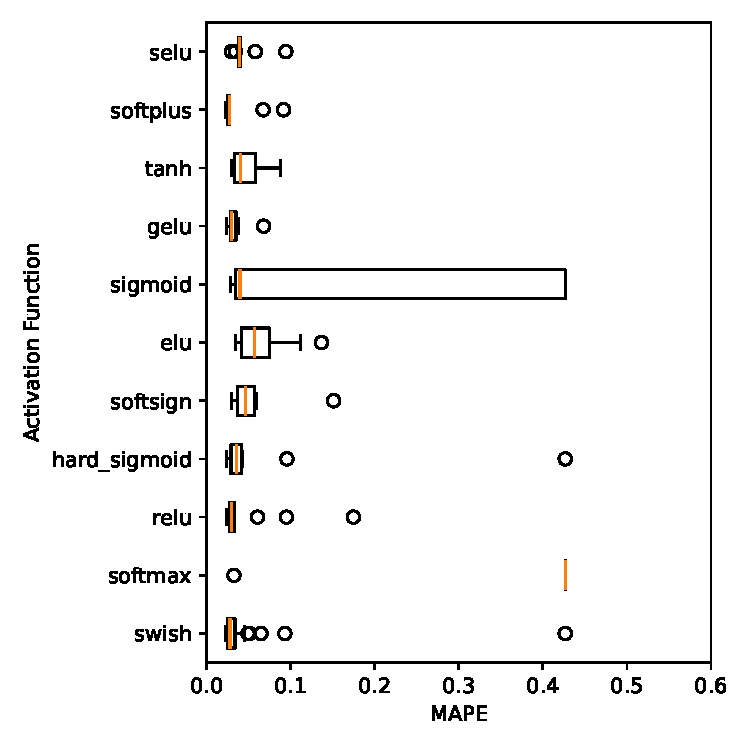
\includegraphics[width=\linewidth]{Figuras/hpo/hpo_plots_#1_#2/hpo_nn_activation_MAPE.pdf}  
        \caption{MAPE.}
        \label{fig:hpo_MAPE_a#1_#2}
    \end{subfigure}
    \begin{subfigure}{0.3\textwidth}
        \centering
        % include second image
        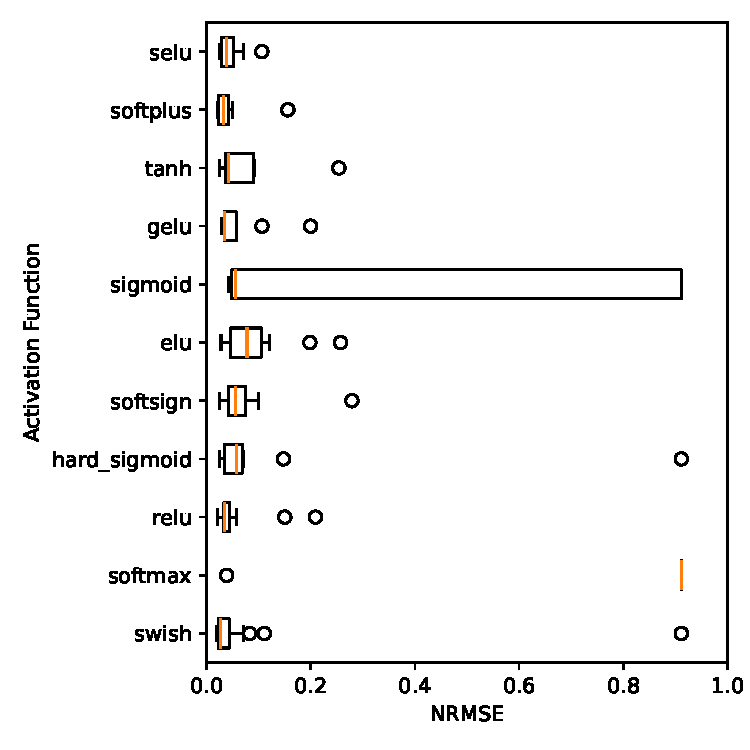
\includegraphics[width=\linewidth]{Figuras/hpo/hpo_plots_#1_#2/hpo_nn_activation_NRMSE.pdf}  
        \caption{NRMSE.}
        \label{fig:hpo_NRMSE_#1_#2}
    \end{subfigure}
    \begin{subfigure}{0.3\textwidth}
        \centering
        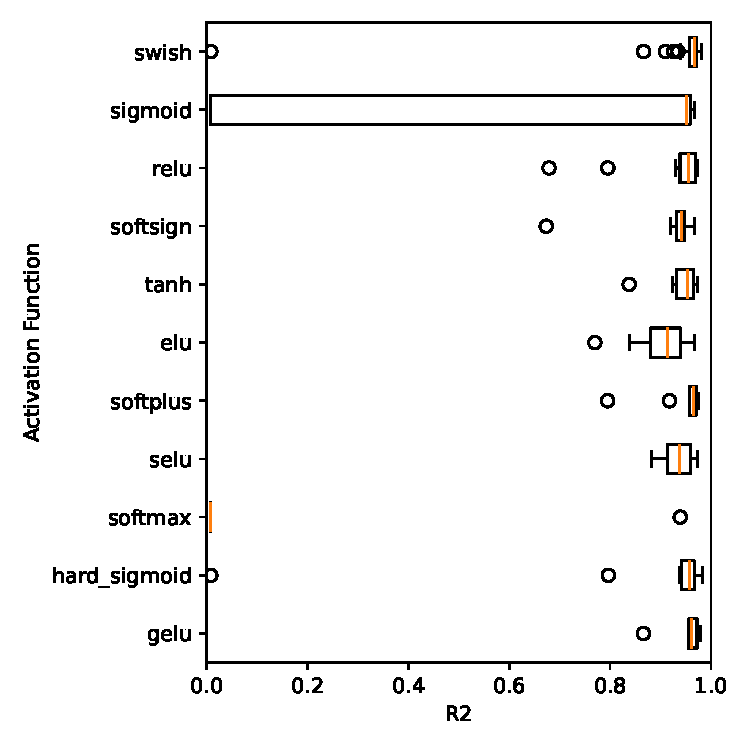
\includegraphics[width=\linewidth]{Figuras/hpo/hpo_plots_#1_#2/hpo_nn_activation_R2.pdf}  
        \caption{R2}
        \label{fig:hpo_R2_#1_#2}
    \end{subfigure}
    \caption{#3}
    \label{fig:hpo_#1_#2}
\end{figure}
}

\newcommand{\plothpomap}[3]{
\begin{figure}[t]
    \centering
    \begin{subfigure}{0.3\textwidth}
        \centering
        % include second image
        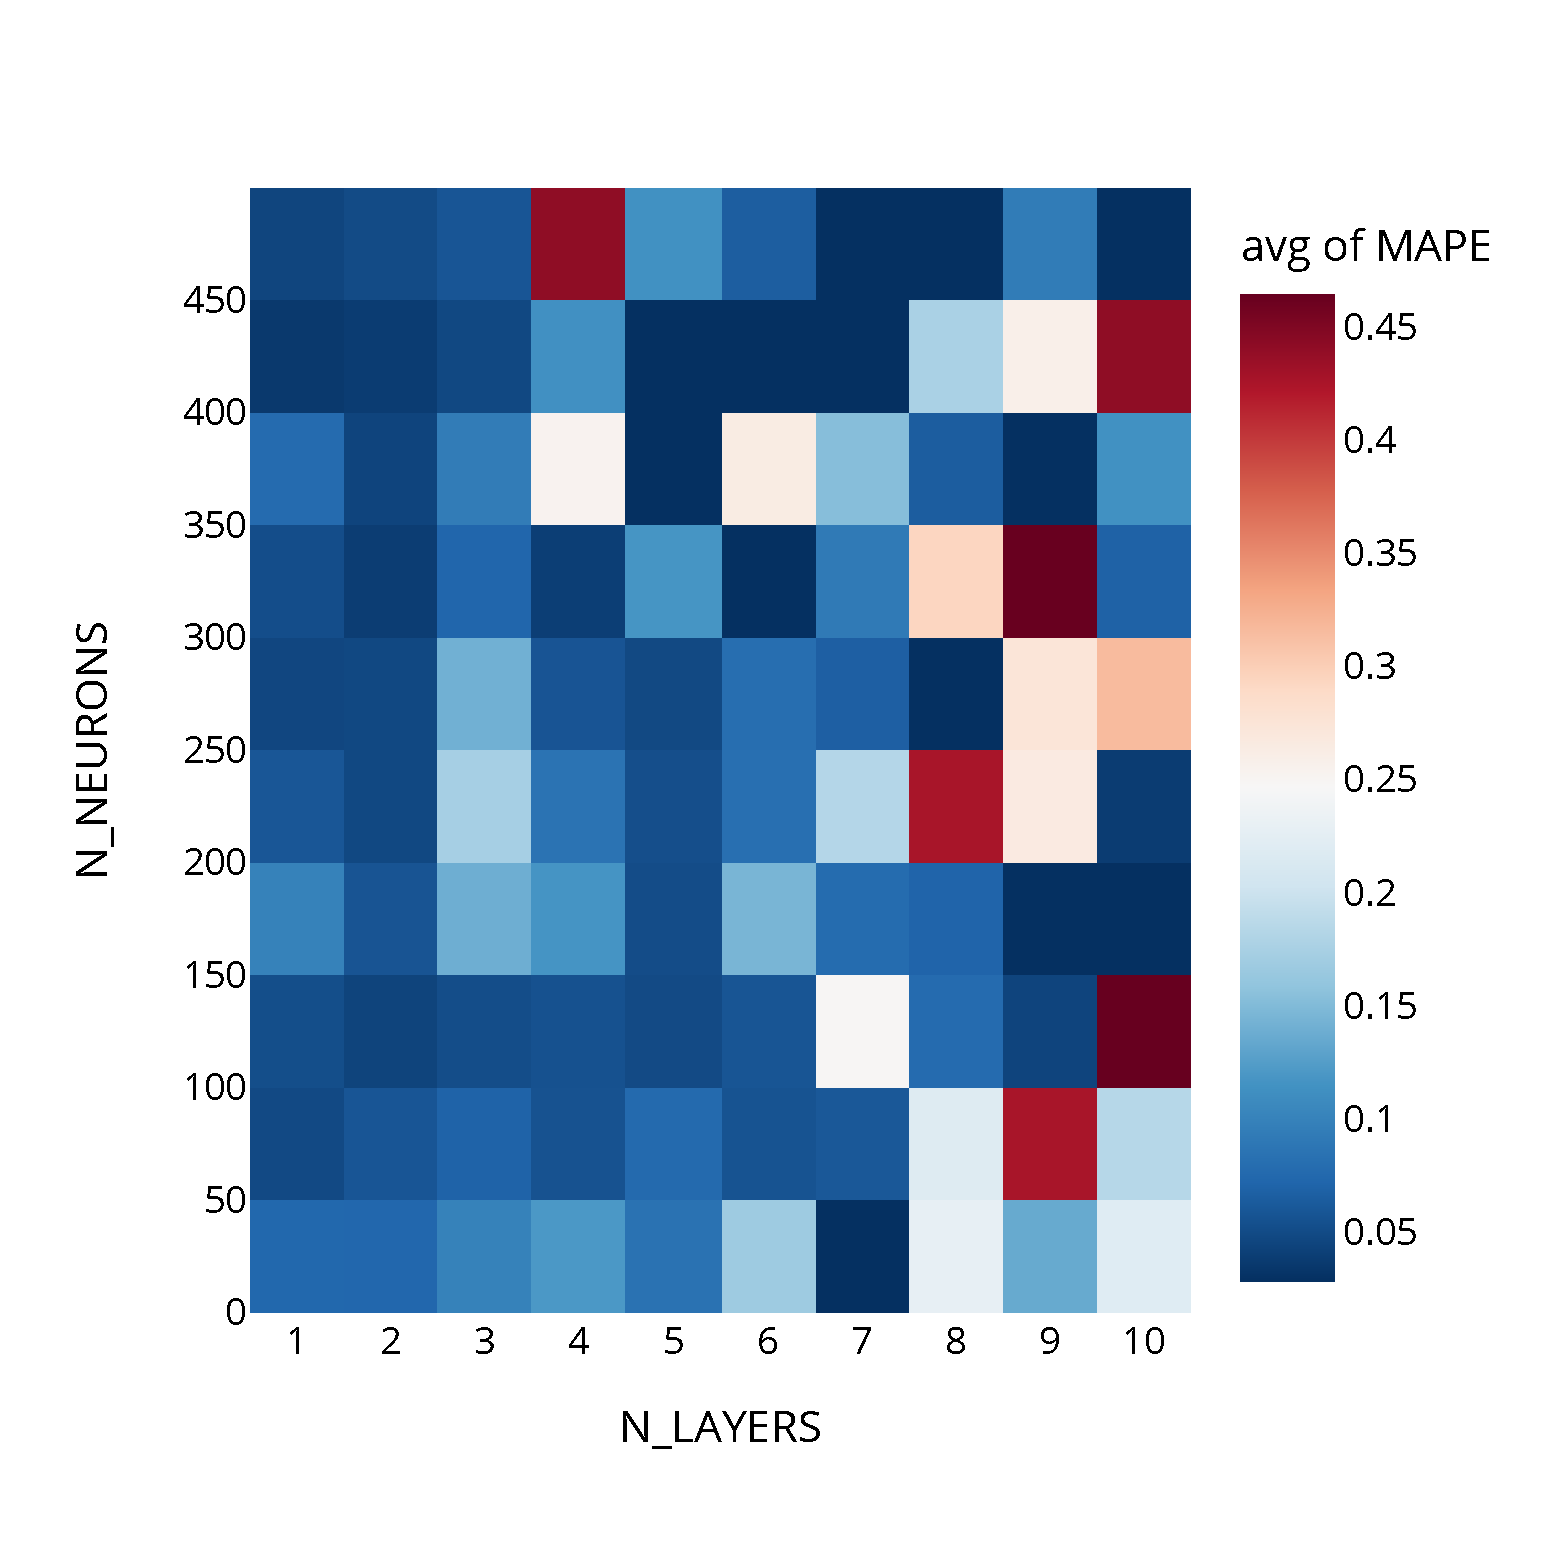
\includegraphics[width=\linewidth]{Figuras/hpo/hpo_plots_#1_#2/neurons_layers_heat_map_MAPE.pdf}  
        \caption{MAPE.}
        \label{fig:hpo_map_MAPE_all_all}
    \end{subfigure}
    \begin{subfigure}{0.3\textwidth}
        \centering
        % include second image
        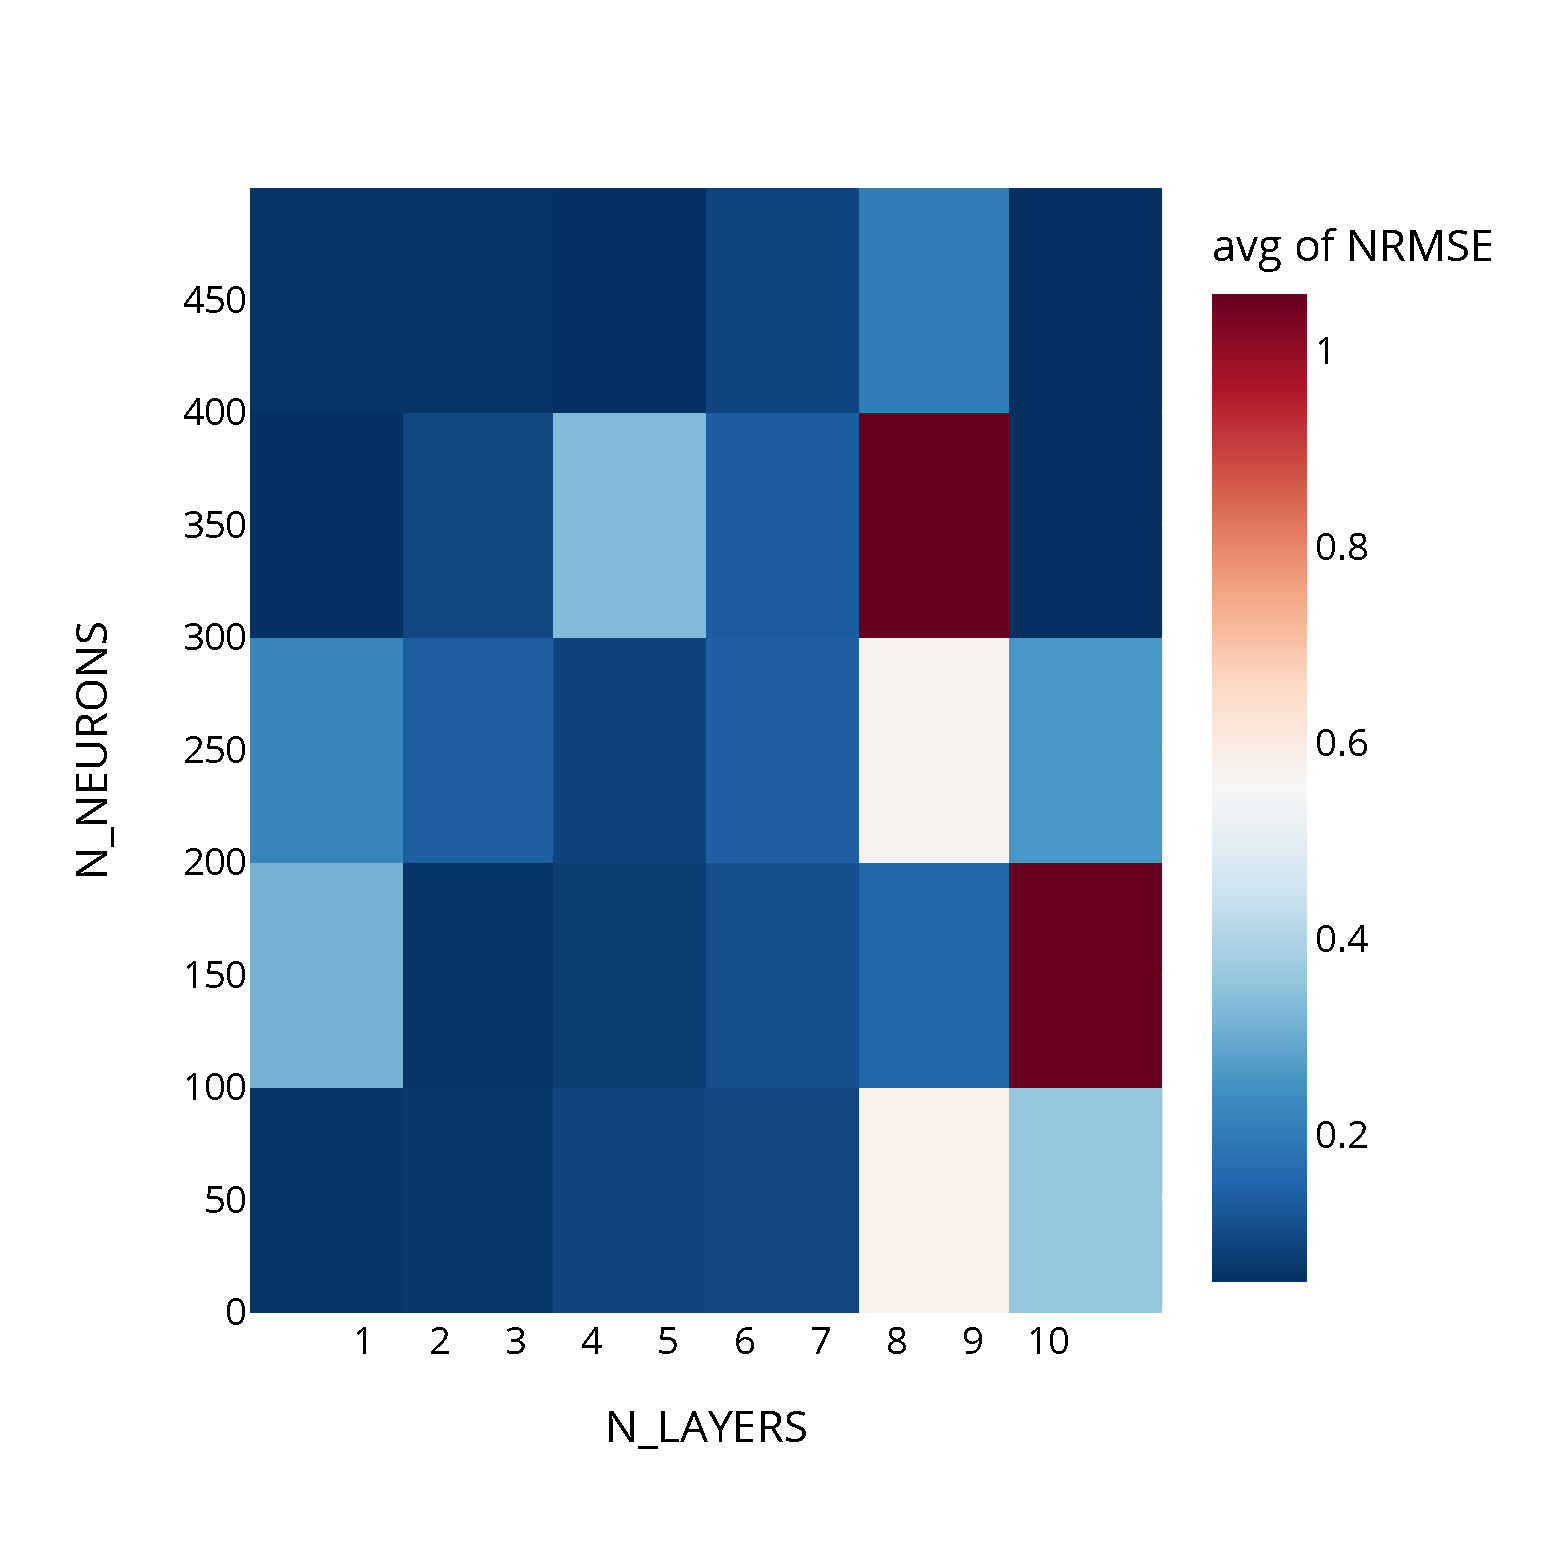
\includegraphics[width=\linewidth]{Figuras/hpo/hpo_plots_#1_#2/neurons_layers_heat_map_NRMSE.pdf}  
        \caption{NRMSE.}
        \label{fig:hpo_map_NRMSE_all_all}
    \end{subfigure}
    \begin{subfigure}{0.3\textwidth}
        \centering
        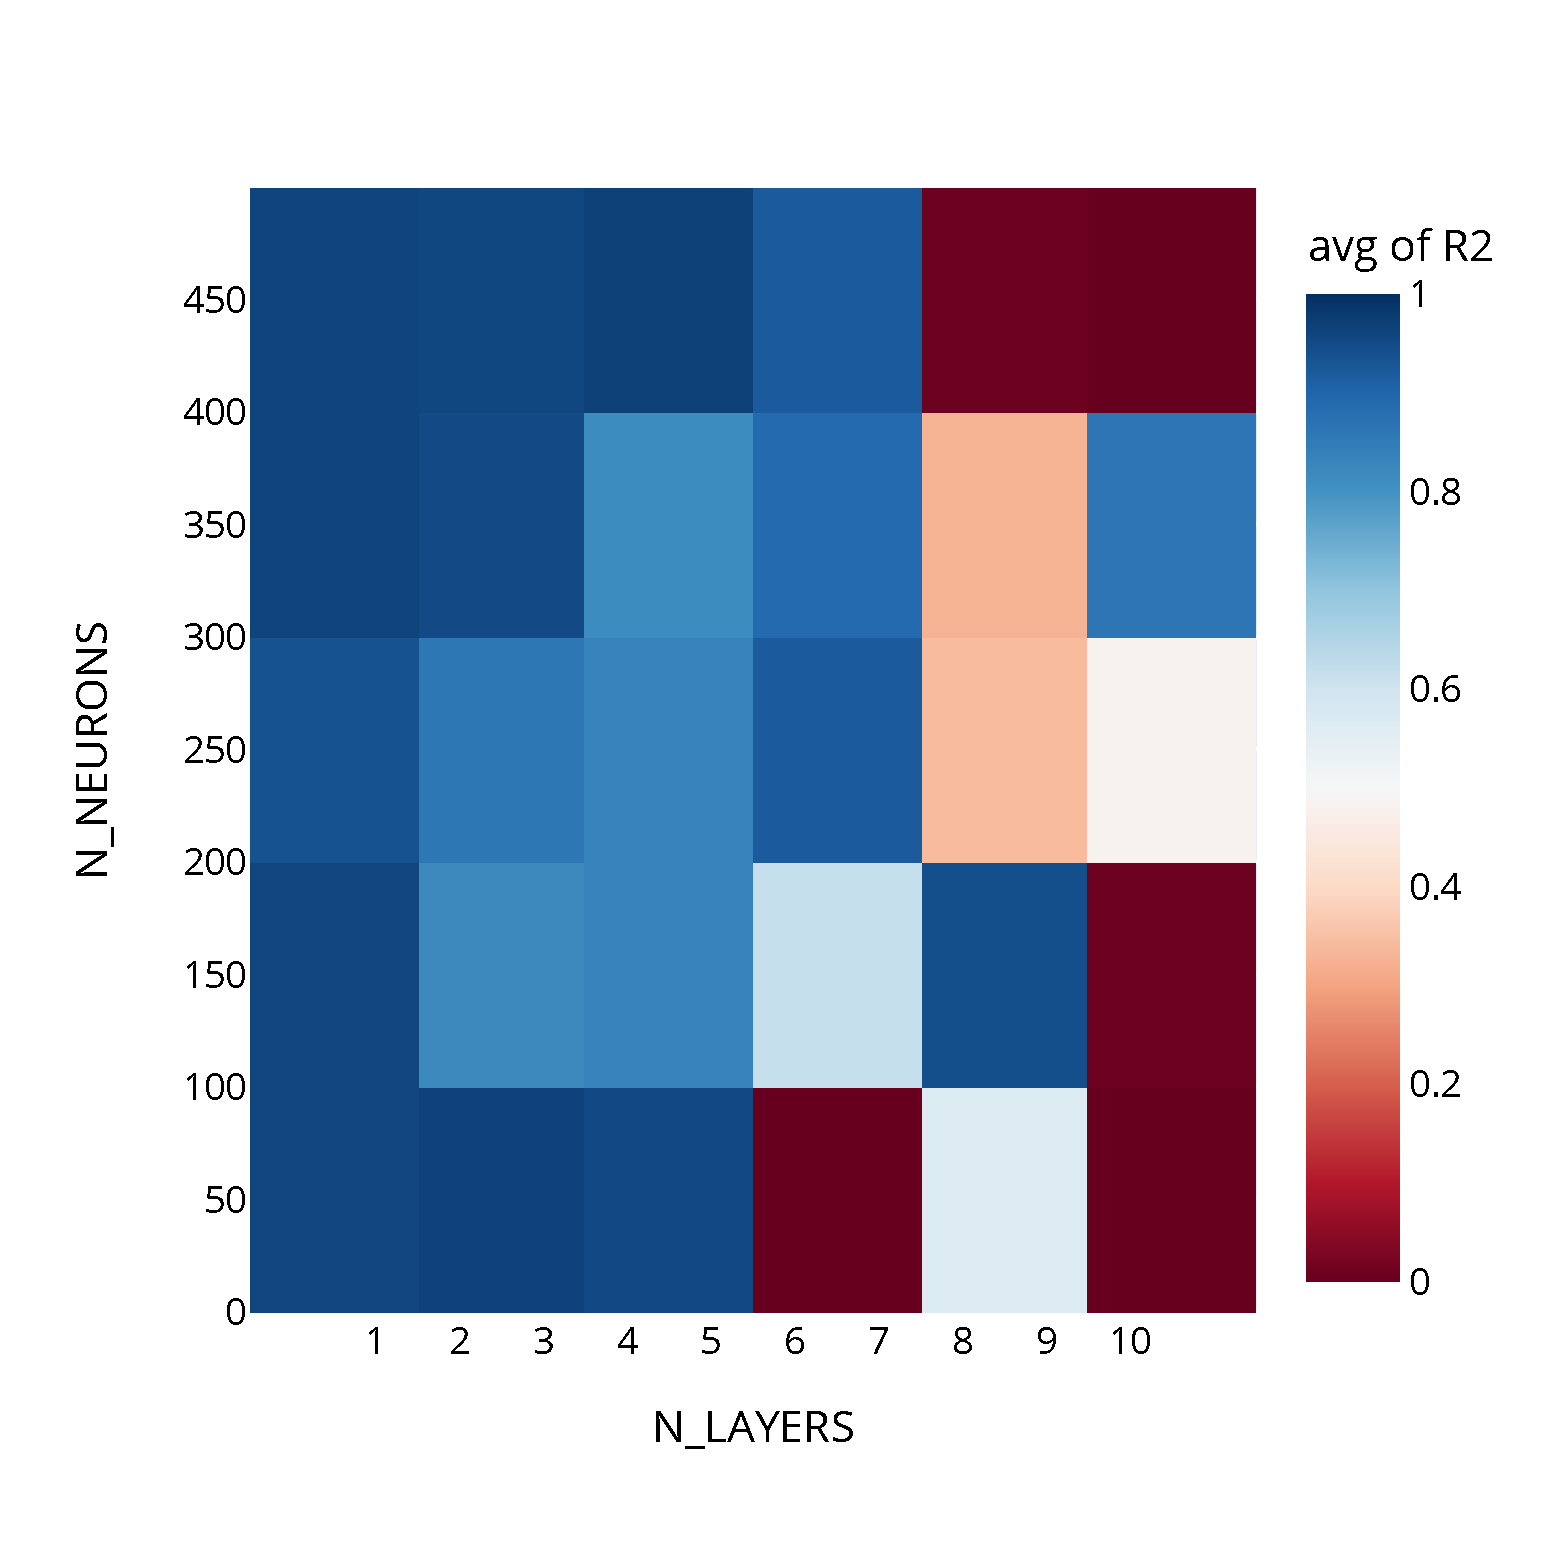
\includegraphics[width=\linewidth]{Figuras/hpo/hpo_plots_#1_#2/neurons_layers_heat_map_R2.pdf}  
        \caption{R2}
        \label{fig:hpo_map_R2_all_all}
    \end{subfigure}
    \caption{#3}
    \label{fig:hpo_map_all_all}
\end{figure}
}

\newcommand{\plothpohistogram}[3]{
\begin{figure}[t]
    \centering
    \begin{subfigure}{0.3\textwidth}
        \centering
        % include second image
        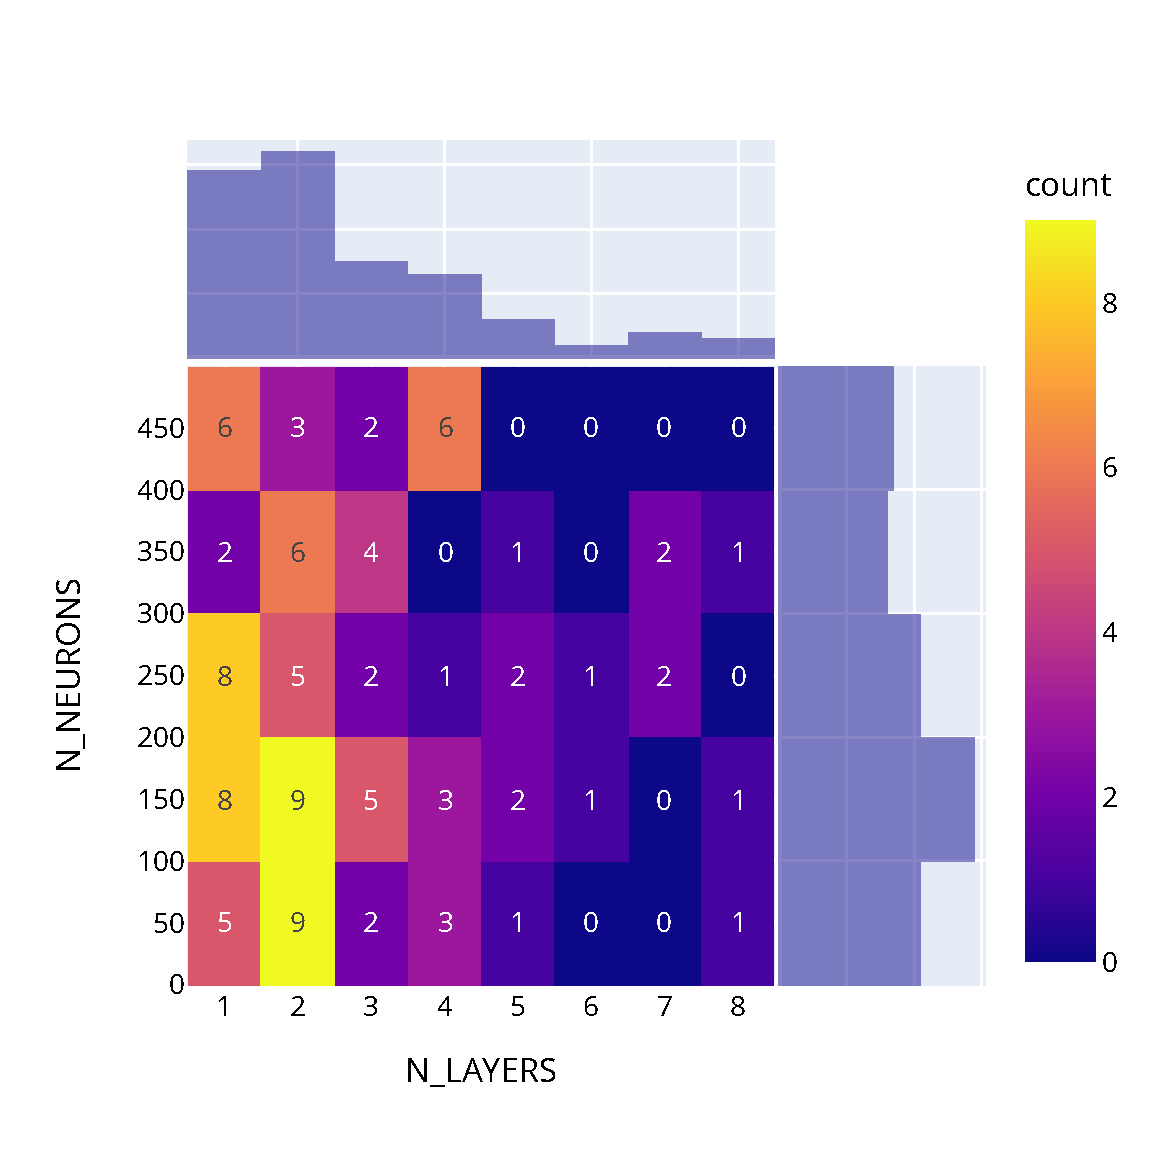
\includegraphics[width=\linewidth]{Figuras/hpo/hpo_plots_#1_#2/hpo_nn_hist_neurons_layers.pdf}  
        \caption{Histogram neurons layers.}
        \label{fig:hpo_hist_neurons_#1_#2}
    \end{subfigure}
    \begin{subfigure}{0.3\textwidth}
        \centering
        % include second image
        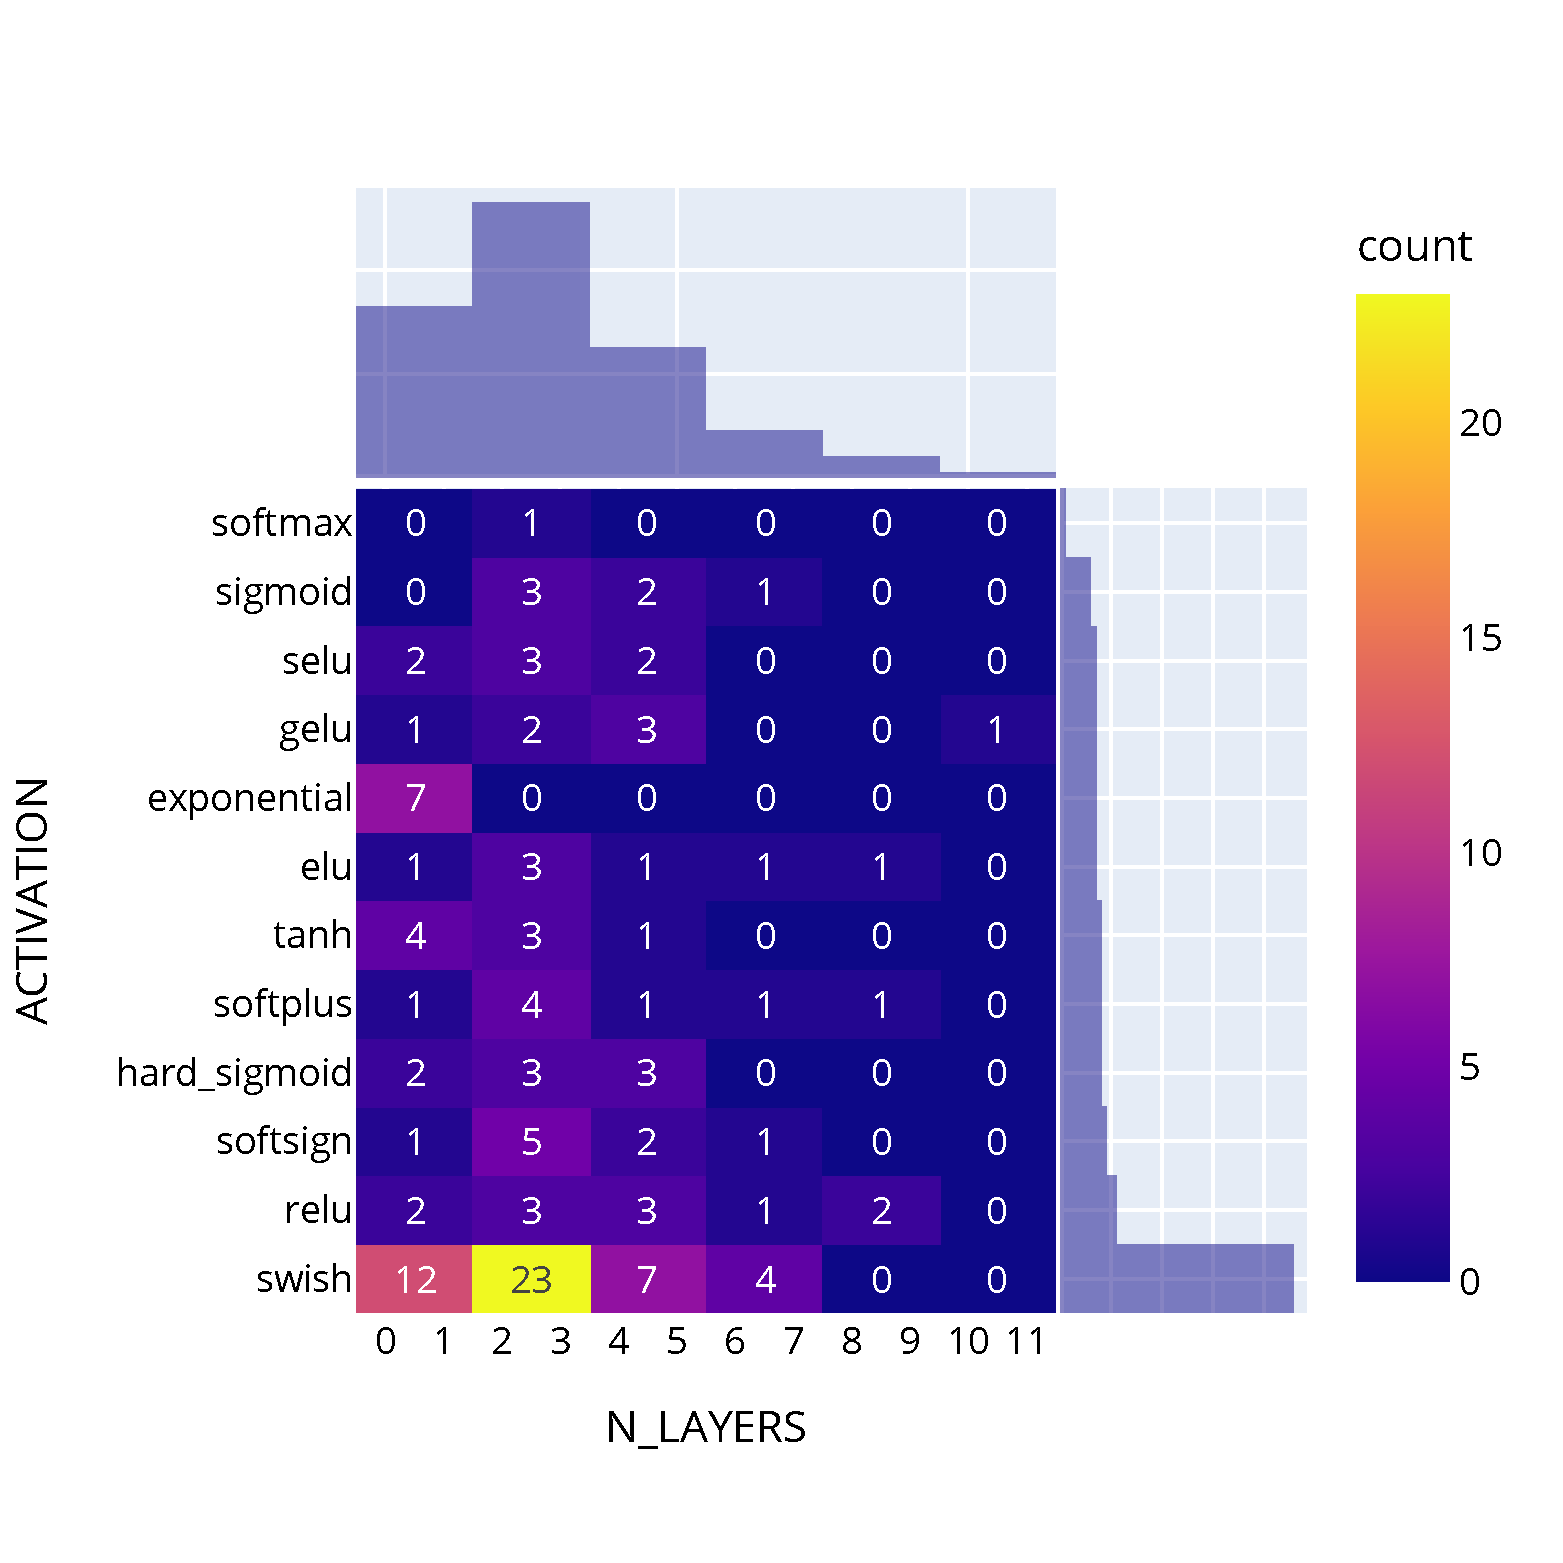
\includegraphics[width=\linewidth]{Figuras/hpo/hpo_plots_#1_#2/hpo_nn_activation_layers_count.pdf}  
        \caption{Histogram activation layers.}
        \label{fig:hpo_hist_activation_#1_#2}
    \end{subfigure}
    \begin{subfigure}{0.3\textwidth}
        \centering
        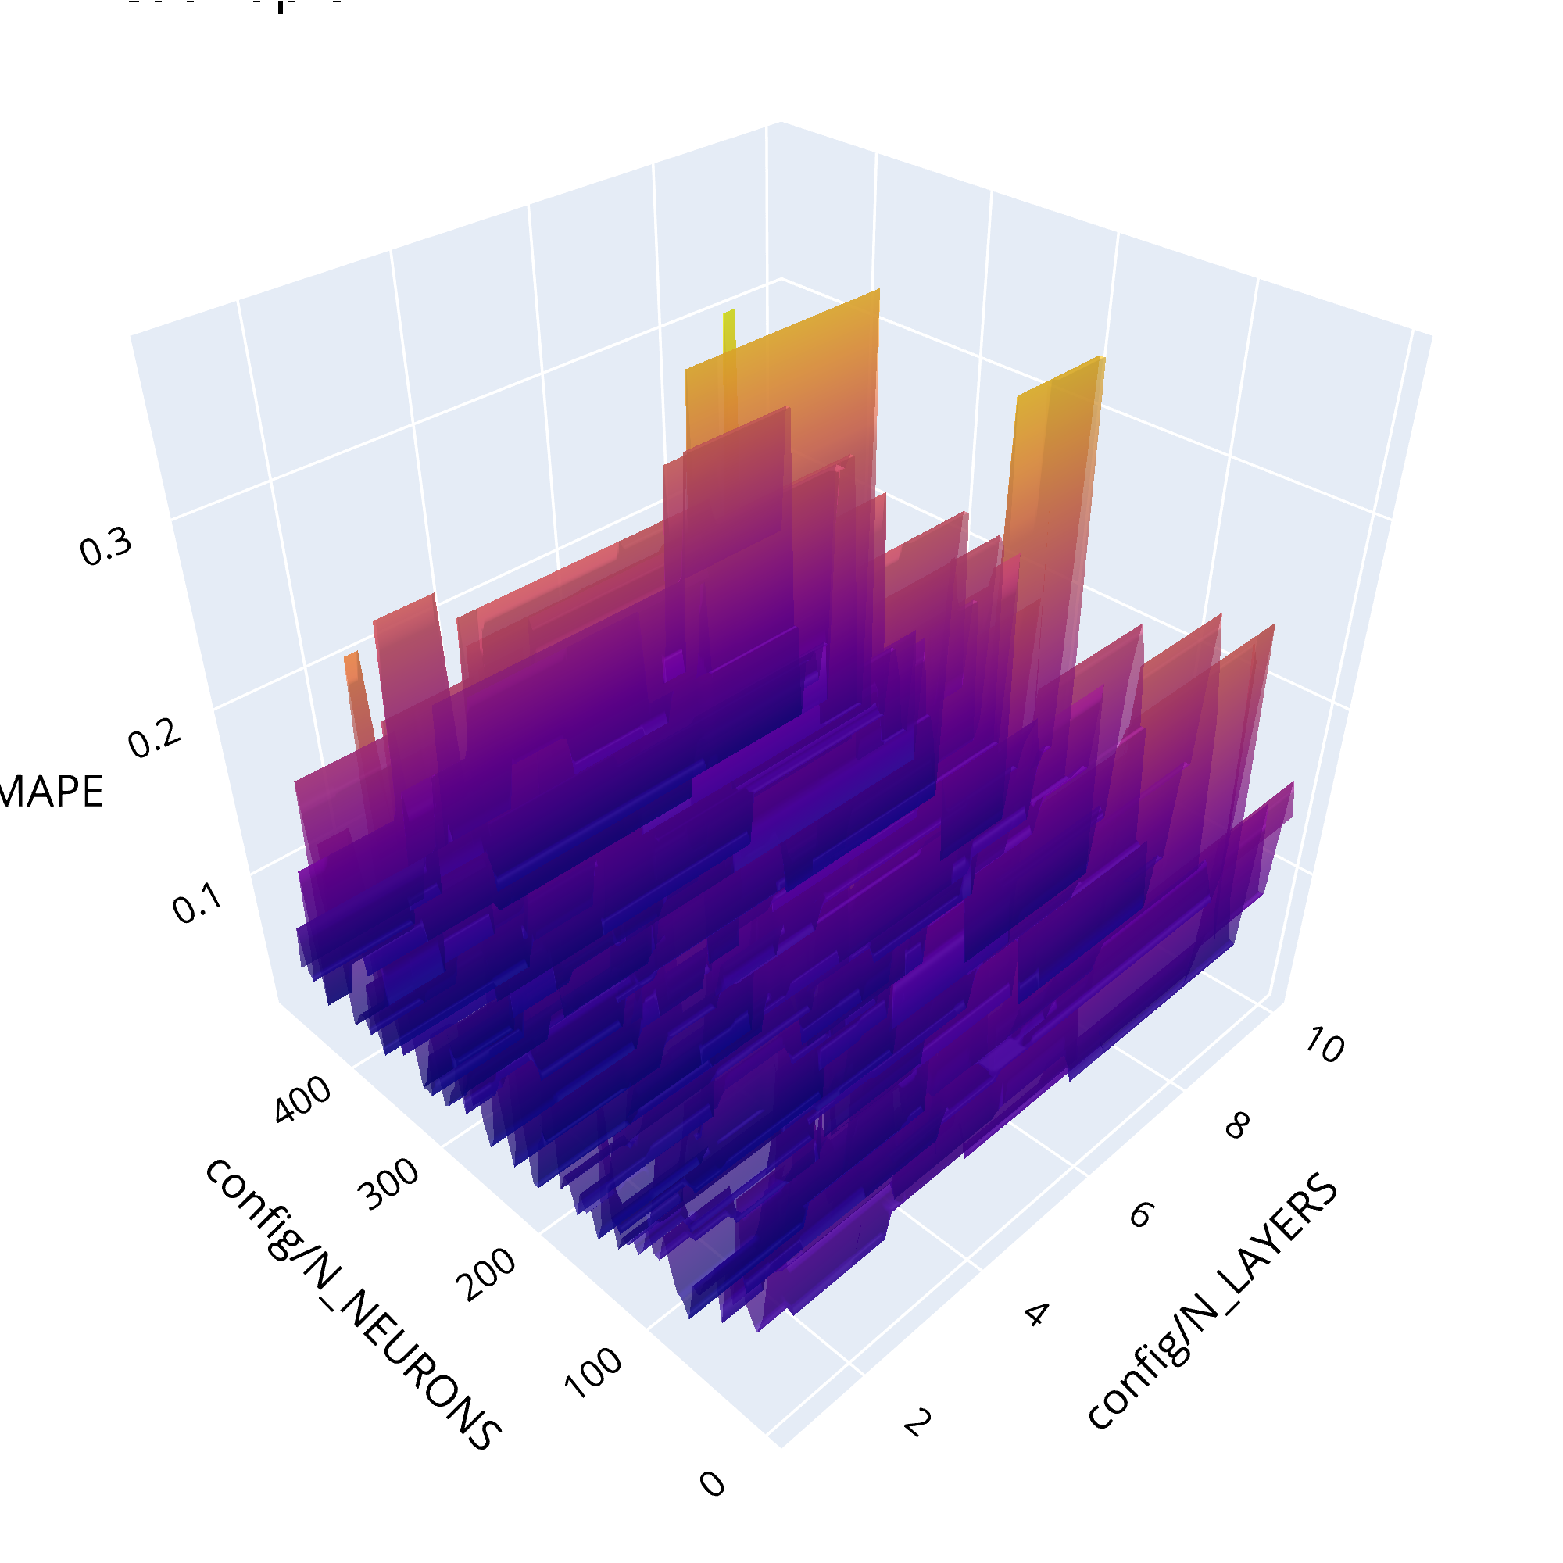
\includegraphics[width=\linewidth]{Figuras/hpo/hpo_plots_#1_#2/hpo_nn_activation_layers_surface.pdf}  
        \caption{Surface MAPE}
        \label{fig:hpo_surface_MAPE_#1_#2}
    \end{subfigure}
    \caption{#3}
    \label{fig:hpo_hist_#1_#2}
\end{figure}
}
%% =============================
%%      IMPORTANTE
%% ESTE ARQUIVO DEVE ESTAR SALVO COMO
%%      UTF - 8
%% =============================

% ----------------------------------------------------------
% Este capítulo é parte integrante do arquivo mestre
% Relatorio_TCC_Mestrado_Base_VERSÃO_SUBVERSÃO
% Formatos com \caption acima do \includegraphics conforme ABNT
% ----------------------------------------------------------

% -----------------------------------------
% Metodologia
%
% A ideia é utilizar a mesma sequência de entrada ter a opção de trocar a posição conforme a necessidade
% 
% O comando deve ser usado dentro do ambiente {figure} de forma que o comando \label{key} esteja dentro do ambiente e permita a melhor localização pelo editor LaTeX
%
% Forma de uso
%
% --------------------- Figuras Simples
%	\begin{figure}[H]
%		\figNameCommand{options includegraphics}{filename with path}{caption}
%		\label{label_figure_1}
%	\end{figure}
%
% --------------------- Figuras Compostas
%	\begin{figure}[H]
%		\figCapTwoSubfigInc{caption geral}
%		{subcaption (a) }
%		{width = 7cm, height = 6cm, trim = 0cm 0cm 0cm 0cm, clip = true}
%		{figure with path}
%		{subcaption (b) }
%		{width = 7cm, height = 6cm, trim = 0cm 0cm 0cm 0cm, clip = true}
%		{figure with path}
%		\label{fig_label}
%	\end{figure}
%
% --------------------- Comando Trim
% trim = left bottom right top
% -----------------------------------------

% -----------------------------------------
% Comandos para Figuras Simples
% -----------------------------------------
\newcommand{\figIncLongCap}[3]
{ 	
	\centering
	\caption{#3}
	\includegraphics[#1]{#2}
}

\newcommand{\figIncShortCap}[4]
{ 	
	\centering
	\caption[#4]{#3}
	\includegraphics[#1]{#2}
}

% -----------------------------------------
% Comandos para Figuras Duplas Com Subfigures
% -----------------------------------------
\newcommand{\figTwoSubfigIncLongCap}[7]
{ 	
	\centering
	\caption{#7}
	\subfigure[#1]
	{\includegraphics[#2]{#3}}
	\quad
	\subfigure[#4]
	{\includegraphics[#5]{#6}}
}

\newcommand{\figTwoSubfigIncShortCap}[8]
{ 	
	\centering
	\caption[#8]{#7}
	\subfigure[#1]
	{\includegraphics[#2]{#3}}
	\quad
	\subfigure[#4]
	{\includegraphics[#5]{#6}}
}

% -----------------------------------------
% Comandos para Figuras Triplas em Cascata Com Subfigures
% -----------------------------------------
\newcommand{\figThreeSubfigIncCap}[4]
{ 	
	\centering
	\SubfigSubcapSubfigInc{#1}
	\quad
	\SubfigSubcapSubfigInc{#2}
	\quad
	\SubfigSubcapSubfigInc{#3}
	\quad
	\caption{#4}
}

% -----------------------------------------
% Comandos Base para Figuras Múltiplas em Cascata Com Subfigures
% -----------------------------------------
\newcommand{\SubfigcapSubfigInc}[3]
{ 	
	\subfigure[#1]
	{\includegraphics[#2]{#3}} 
}

%%%%%%%%%%%%%%%%%%%%%%%%%%%%%%%%%%
% ===== Magno old versions ===== %
%%%%%%%%%%%%%%%%%%%%%%%%%%%%%%%%%%

% -----------------------------------------
% Comandos para Figuras Duplas sem Subfigure
% -----------------------------------------
\newcommand{\figDob}[5]
{   
	\centering
	\caption{#5}
	\includegraphics[#1]{#2}
	\includegraphics[#3]{#4} \\
	\vspace*{0.2cm}
	(a) \hspace{6.5cm} (b)
}

% -----------------------------------------
% Comandos para Figuras Triplas sem Subfigure
% -----------------------------------------
\newcommand{\figTre}[7]
{   
	\centering
	\caption{#7}
	\includegraphics[#1]{#2}
	\includegraphics[#3]{#4} \\
	\vspace*{0.2cm}
	(a) \hspace{6.5cm} (b) \\
	\includegraphics[#5]{#6} \\
	\vspace*{0.2cm}
	(c)
}

\newcommand{\figTreV}[7]
{   
	\centering
	\caption{#7}
	\includegraphics[#1]{#2}
	\includegraphics[#3]{#4}
	\includegraphics[#5]{#6}   \\
	\vspace*{0.2cm}
	(a) \hspace{4.cm} (b) \hspace{4.cm} (c)
}
% ----------------------------------------------------------
% Fim Arquivo
%%% =============================
%%      IMPORTANTE
%% ESTE ARQUIVO DEVE ESTAR SALVO COMO
%%      UTF - 8
%% =============================

% ----------------------------------------------------------
% Este capítulo é parte integrante do arquivo mestre
% Relatorio_TCC_Mestrado_Base_VERSÃO_SUBVERSÃO
% Formatos com \caption acima do \includegraphics conforme todos exceto ABNT, e.g., IEEE
% ----------------------------------------------------------

% -----------------------------------------
% Metodologia
%
% A ideia é utilizar a mesma sequência de entrada ter a opção de trocar a posição conforme a necessidade
% 
% O comando deve ser usado dentro do ambiente {figure} de forma que o comando \label{key} esteja dentro do ambiente e permita a melhor localização pelo editor LaTeX
%
% Forma de uso
%
% --------------------- Figuras Simples
%	\begin{figure}[H]
%		\figNameCommand{options includegraphics}{filename with path}{caption}
%		\label{label_figure_1}
%	\end{figure}
%
% --------------------- Figuras Compostas
%	\begin{figure}[H]
%		\figCapTwoSubfigInc{caption geral}
%		{subcaption (a) }
%		{width = 7cm, height = 6cm, trim = 0cm 0cm 0cm 0cm, clip = true}
%		{figure with path}
%		{subcaption (b) }
%		{width = 7cm, height = 6cm, trim = 0cm 0cm 0cm 0cm, clip = true}
%		{figure with path}
%		\label{fig_label}
%	\end{figure}
%
% --------------------- Comando Trim
% trim = left bottom right top
% -----------------------------------------

% -----------------------------------------
% Comandos para Figuras Simples
% -----------------------------------------
\newcommand{\figIncLongCap}[3]
{ 	
	\centering
	\includegraphics[#1]{#2}
	\caption{#3}
}

\newcommand{\figIncShortCap}[4]
{ 	
	\centering
	\includegraphics[#1]{#2}
	\caption[#4]{#3}
}

% -----------------------------------------
% Comandos para Figuras Duplas Com Subfigures
% -----------------------------------------
\newcommand{\figTwoSubfigIncLongCap}[7]
{ 	
	\centering
	\subfigure[#1]
	{\includegraphics[#2]{#3}}
	\quad
	\subfigure[#4]
	{\includegraphics[#5]{#6}}
	\caption{#7}
}

\newcommand{\figTwoSubfigIncShortCap}[8]
{ 	
	\centering
	\subfigure[#1]
	{\includegraphics[#2]{#3}}
	\quad
	\subfigure[#4]
	{\includegraphics[#5]{#6}}
	\caption[#8]{#7}
}

% -----------------------------------------
% Comandos para Figuras Triplas em Cascata Com Subfigures
% -----------------------------------------
\newcommand{\figThreeSubfigIncCap}[4]
{ 	
	\centering
	\SubfigSubcapSubfigInc{#1}
	\quad
	\SubfigSubcapSubfigInc{#2}
	\quad
	\SubfigSubcapSubfigInc{#3}
	\quad
	\caption{#4}
}

% -----------------------------------------
% Comandos Base para Figuras Múltiplas em Cascata Com Subfigures
% -----------------------------------------
\newcommand{\SubfigcapSubfigInc}[3]
{ 	
	\subfigure[#1]
	{\includegraphics[#2]{#3}} 
}

%%%%%%%%%%%%%%%%%%%%%%%%%%%%%%%%%%
% ===== Magno old versions ===== %
%%%%%%%%%%%%%%%%%%%%%%%%%%%%%%%%%%

% -----------------------------------------
% Comandos para Figuras Duplas sem Subfigure
% -----------------------------------------
\newcommand{\figDob}[5]
{   
	\centering
	\includegraphics[#1]{#2}
	\includegraphics[#3]{#4} \\
	\vspace*{0.2cm}
	(a) \hspace{6.5cm} (b) %\\
	\caption{#5}
}

% -----------------------------------------
% Comandos para Figuras Triplas sem Subfigure
% -----------------------------------------
\newcommand{\figTre}[7]
{   
	\centering
	\includegraphics[#1]{#2}
	\includegraphics[#3]{#4} \\
	\vspace*{0.2cm}
	(a) \hspace{6.5cm} (b) \\
	\includegraphics[#5]{#6} \\
	\vspace*{0.2cm}
	(c)
	\caption{#7}
}

\newcommand{\figTreV}[7]
{   
	\centering
	\includegraphics[#1]{#2}
	\includegraphics[#3]{#4}
	\includegraphics[#5]{#6}   \\
	\vspace*{0.2cm}
	(a) \hspace{4.cm} (b) \hspace{4.cm} (c)
	\caption{#7}
}
% ----------------------------------------------------------
% Fim Arquivo

% ==========

% ==========  Seleção de uso de links coloridos para visualização ou sem cor para impressão final
%\toggletrue{LinksComCores} 		% Opção links COM CORES => Forma para auxiliar na escrita do relatório
\togglefalse{LinksComCores} 		% Opção links SEM CORES => Forma correta para imprimir a versão final a ser entregue
% ==========

% ========== Pacotes
%% =============================
%%      IMPORTANTE
%% ESTE ARQUIVO DEVE ESTAR SALVO COMO
%%      UTF - 8
%% =============================

% ----------------------------------------------------------
% Este capítulo é parte integrante do arquivo mestre
% Relatorio_TCC_Mestrado_Base_VERSÃO_SUBVERSÃO
% ----------------------------------------------------------
\usepackage{natbib}
\usepackage[T1]{fontenc}
%\usepackage[latin1]{inputenc}
\usepackage[utf8]{inputenc}
% =========
\usepackage{pgfplots}
\usepackage{tabularx}
% -----------------------------------------
% Pacotes básicos 
% -----------------------------------------
\usepackage[section]{placeins}
\usepackage{lastpage}		% Usado pela Ficha catalográfica
\usepackage{indentfirst}	% Indenta o primeiro parágrafo de cada seção.
\usepackage{color}			% Controle das cores
\usepackage{microtype} 		% Melhorias de justificação \usepackage[section]{placeins}
% \usepackage{amsmath} 		% Referências de equações com parênteses automático usar \eqref
\usepackage{physics,amsmath}

\usepackage{amssymb} 		% Símbolos matemáticos, incluindo os principais conjuntos numéricos
\usepackage{cancel}
% -----------------------------------------

% -----------------------------------------
% Pacotes gráficos
% -----------------------------------------
\usepackage{ae}
\usepackage{aecompl}
\usepackage{graphicx, import}	% Inclusão de gráficos
\usepackage{float} 		% Permite que eu use "H" para a figura ficar entre os parágrafos que eu quero
%\usepackage{subfigure} % make it possible to include more than one captioned figure/table in a single float
%\usepackage[font=small,labelfont=bf]{caption}
\usepackage[font=footnotesize]{caption} % Reduz o tamanho de todos os ``captions''
%\usepackage{subcaption}
%\usepackage{subfloat} % make it possible to include more than one captioned 
\usepackage{epstopdf}
\usepackage{ulem}
\usepackage{nomencl}
\makenomenclature
% \usepackage{framed}
\usepackage{lipsum} % geração de texto inútil - dummy
\usepackage{morefloats}

% -----------------------------------------
% Pacotes gráficos - Formatação do título
% -----------------------------------------
% Se fncychap for adicionado como RequirePackage dentro de ufabcFHZ#.cls não gera o mesmo efeito.
\usepackage[Bjornstrup]{fncychap} % Formas elegantes de cabeçalho
%% ------------------------------------
% Referência: http://tex.stackexchange.com/questions/13357/fncychap-package-reduce-vertical-gap-space-between-header-and-chapter-heading
%% ------------------------------------
%% A única alteração feita é em ``\vspace'', por padrão será usado ``-1cm'', fica bom, maximiza o espaço  - Não é necessário editar esse trecho.
%% ------------------------------------
\makeatletter
\renewcommand*{\@makechapterhead}[1]{%
	%\vspace*{-5\p@}%
	\vspace*{-1cm}% Recuo vertical para maximizar aproveitamento da página
	{\parindent \z@ \raggedright \normalfont
		\ifnum \c@secnumdepth >\m@ne
		\if@mainmatter%%%%% Fix for frontmatter, mainmatter, and backmatter 040920
		\DOCH
		\fi
		\fi
		\interlinepenalty\@M
		\if@mainmatter%%%%% Fix for frontmatter, mainmatter, and backmatter 060424
		\DOTI{#1}%
		\else%
		\DOTIS{#1}%
		\fi
	}
}
% For the case \chapter*:
\renewcommand*{\@makeschapterhead}[1]{%
	\vspace*{-1cm}% Recuo vertical para maximizar aproveitamento da página
	{\parindent \z@ \raggedright
		\normalfont
		\interlinepenalty\@M
		\DOTIS{#1}
		\vskip 40\p@
	}
}
\makeatother
%% ------------------------------------

% -----------------------------------------
% Pacotes Ambiente de comentário
% -----------------------------------------
\usepackage{comment}

% ----------------------------------------- 
% Tabelas
% ----------------------------------------- 
\usepackage{booktabs} % for much better looking tables
\usepackage{multirow} % Permite uma célula de várias linhas
% ----------------------------------------- 

% ----------------------------------------- 
% Enumerate com letras pré-fixas
% ----------------------------------------- 
\usepackage{paralist} 		% very flexible & customisable lists (eg. enumerate/itemize, etc.)
\usepackage{enumitem}

% ----------------------------------------- 
% Equações
% ----------------------------------------- 
\usepackage{breqn} 		 % Garante quebra automático com \begin{dmath}, mesmo contador de \begin{equation}
\usepackage{array} 		 % for better arrays (eg matrices) in maths
\usepackage{subeqnarray} % Permite o use de subnumeração numa equação 1.a 1.b 1.c etc
\usepackage{cancel} 	 % Permite o corte numa simplificação de expressão:
% \cancel{expression}
% \cancelto{value}{expression}

% ----------------------------------------- 
% Links Coloridos - Com seleção de uso de cores pelo usuário no arquivo base usando \toogletrue ou \togglefalse
% ----------------------------------------- 
\usepackage[colorlinks=true,
linkcolor 		= red,
anchorcolor 	= black,
citecolor 		= green,
filecolor 		= cyan,
	% ==== Selecionando opção de links coloridos - Em parceria com comando "\newtoggle{LinksComCores}"
	\iftoggle{LinksComCores}{%
		%hidelinks
	}{%
		hidelinks
	}
	% ==== 
]{hyperref} %Pacote para hyperlinks
%hidelinks %opção para os links não serem coloridos, útil para a versão final do trabalho, também posso usar %linkcolor=black


% ----------------------------------------- 
% Links Coloridos - Com seleção de uso de cores (des)comentando "hidelinks"
%% - Este código está dentro da classe ufabcFHZ#.cls
%% - 	Ele é mantido aqui para conferência
% ----------------------------------------- 
%\usepackage[colorlinks=true,
%linkcolor 		= red,
%anchorcolor 	= black,
%citecolor 		= green,
%filecolor 		= cyan,
%hidelinks
%]{hyperref} %Pacote para hyperlinks
%%hidelinks %opção para os links não serem coloridos, útil para a versão final do trabalho, também posso usar %linkcolor=black

% ----------------------------------------- 
% Inserção de código do Matlab
% ----------------------------------------- 
\usepackage[numbered]{mcode} 		% configure listings for Matlab

%==== Pacote para url nas referências da ABNT
%\usepackage[num,abnt-url-package=url]{abntcite}
%====

% for subfigures
\usepackage{caption}
\usepackage{subcaption}
\usepackage{capt-of}

% to draw circuits
\usepackage{circuitikz}
\usepackage{tikz}

\usepackage{makecell}
% ----------------------------------------------------------
% Fim Arquivo

\usetikzlibrary{shapes.geometric,arrows.meta}
\usetikzlibrary{positioning}
\usetikzlibrary{calc}
\usetikzlibrary{backgrounds}
\usetikzlibrary{fit}

\tikzstyle{diam} = [diamond, aspect=2, draw, fill=red!40, text width=6em,text centered ]
\tikzstyle{block} = [rectangle, draw, fill=blue!20, text width=3cm,text centered, rounded corners, minimum height=2em ]
\tikzstyle{trap} = [trapezium, trapezium left angle=70, trapezium right angle=110, minimum height=2em, text centered, draw=red, fill=green!30]
\tikzstyle{rect} = [rectangle, minimum width=3cm, minimum height=1cm, text centered, draw=red, fill=orange!30]
\tikzstyle{line} = [draw, -latex]


% for pseudo codes
\usepackage{algorithm}
\usepackage[noend]{algpseudocode}

\makeatletter
\newcommand*{\algrule}[1][\algorithmicindent]{%
  \makebox[#1][l]{%
    \hspace*{.2em}% <------------- This is where the rule starts from
    \vrule height .75\baselineskip depth .25\baselineskip
  }
}
\newcount\ALG@printindent@tempcnta
\def\ALG@printindent{%
    \ifnum \theALG@nested>0% is there anything to print
    \ifx\ALG@text\ALG@x@notext% is this an end group without any text?
    % do nothing
    \else
    \unskip
    % draw a rule for each indent level
    \ALG@printindent@tempcnta=1
    \loop
    \algrule[\csname ALG@ind@\the\ALG@printindent@tempcnta\endcsname]%
    \advance \ALG@printindent@tempcnta 1
    \ifnum \ALG@printindent@tempcnta<\numexpr\theALG@nested+1\relax
    \repeat
    \fi
    \fi
}
% the following line injects our new indent handling code in place of the default spacing
\patchcmd{\ALG@doentity}{\noindent\hskip\ALG@tlm}{\ALG@printindent}{}{\errmessage{failed to patch}}
\patchcmd{\ALG@doentity}{\item[]\nointerlineskip}{}{}{} % no spurious vertical space
% end vertical rule patch for algorithmicx
\makeatother

% mathcal lowerletters
%\usepackage{dutchcal}

%\input{Pacotes/Input_Pacotes_for_IEEE}
%%% =============================
%%      IMPORTANTE
%% ESTE ARQUIVO DEVE ESTAR SALVO COMO
%%      UTF - 8
%% =============================

% ----------------------------------------------------------
% Este capítulo é parte integrante do arquivo mestre
% Relatorio_TCC_Mestrado_Base_VERSÃO_SUBVERSÃO
% ----------------------------------------------------------


%================ Pacotes para inserir código
% ----------------------------------------- 
% Inserção de código do Matlab
% ----------------------------------------- 
\usepackage[numbered]{mcode} 		% configure listings for Matlab

% Deve estar na mesma pasta que o arquivo Base do relatório
%%%% *** Bloco adicionado em mcode.sty - FHZ
% % general definitions
% \lstset{%
% extendedchars = true,
% inputencoding = latin1, % funciona com latin1
%%%% ***

% ----------------------------------------- 
% en­ables the user to type­set pro­grams (pro­gram­ming code) 
% ----------------------------------------- 
\usepackage{listings}

%%%%% ++++++ Referências e explicações:
%http://tex.stackexchange.com/questions/68356/how-to-create-conditionals-in-a-document-class-for-latex
%http://tex.stackexchange.com/questions/30512/how-to-insert-code-with-accents-with-listings
%http://tex.stackexchange.com/questions/24528/having-problems-with-listings-and-utf-8-can-it-be-fixed
%http://tex.stackexchange.com/questions/30512/how-to-insert-code-with-accents-with-listings
%http://tex.searchalleasy.com/q/30512
%http://stackoverflow.com/questions/1116266/listings-in-latex-with-utf-8-or-at-least-german-umlauts
%http://www.mathworks.com/matlabcentral/fileexchange/8015-m-code-latex-package
%%%%% ++++++ 

% ----------------------------------------- 
% --- Comando para definir estilo da \lstinputlisting
% ----------------------------------------- 
\lstset{basicstyle=\footnotesize}

% ----------------------------------------- 
% --- Comando para garantir acentuação correta para \lstinputlisting[language = C].
% ----------------------------------------- 
\lstset{literate = %
	{Ö}{{\"O}}1
	{Ä}{{\"A}}1
	{Ü}{{\"U}}1
	{ß}{{\s{s}}}1
	{ü}{{\"u}}1
	{ä}{{\"a}}1
	{ö}{{\"o}}1
	{~}{{\textasciitilde}}1
	{ã}{{\~a}}1
	{á}{{\'a}}1
	{à}{{\`a}}1
	{â}{{\^a}}1
	{é}{{\'e}}1
	{ê}{{\^e}}1
	{í}{{\'\i}}1
	{õ}{{\~o}}1
	{ó}{{\'o}}1
	{ô}{{\^o}}1
	{ú}{{\'u}}1
	{ç}{{\c c}}1
	{Ã}{{\~A}}1
	{Á}{{\'A}}1
	{À}{{\`A}}1
	{Â}{{\^A}}1
	{É}{{\'E}}1
	{Ê}{{\^E}}1
	{Í}{{\'{I}}}1
	{Õ}{{\~O}}1
	{Ó}{{\'O}}1
	{Ô}{{\^O}}1
	{Ú}{{\'U}}1
	{Ç}{{\c {C}}}1
}
%================

% ----------------------------------------------------------
% Fim Arquivo
% ========== 

% ========== Caminho das Figuras
%\graphicspath{{Figuras/}}
%\graphicspath{{Textuais/Images/Fig-Internet.JPG}}
% ========== 

% ------------------------------------------
% Cria Lista de Símbolos
% ------------------------------------------
\makelosymbols

% ------------------------------------------
% Cria Lista de Abreviações
% ------------------------------------------
\makeloabbreviations

% ------------------------------------------
% Início do documento
% ------------------------------------------
\begin{document}
	
% -----------------------------------------
% INFORMAÇÕES E DADOS - CAPA e FOLHA DE ROSTO
% -----------------------------------------

\title{Titulo}


\foreigntitle{English Title}



\author{}{Autor}



% ------- Orientador e (se houver) Coorientador
\advisor{ Prof. Dr.}{Romulo}{Gonçalves Lins}{}
\advisor{ Prof. Dr.}{Ricardo}{Gaspar}{}

% ------- Banca
\examiner{Profa. Dra.}{Marcia Maria Penteado Marchesini}{Examinadora Externa}
\examiner{Prof. Dr.}{Wilson Carlos da Silva Júnior}{Examinador Externo}
\examiner{Profa. Dra.}{Franciane Freitas Silveira}{Examinadora Interna Suplente}
\examiner{Prof. Dr.}{ Rômulo Gonçalves Lins}{Presidente}
% ------- Coordenador do curso
\coordinator{Prof.}{Dr.}{NomeCoordenador}{}
% ------ Data de entrega
\date{23}{03}{2022} % dia - mês - ano
% ------ Limite de 5 palavras chaves para ficha catalográfica
\keyword{K1}
\keyword{K2}
\keyword{K3}
\keyword{K4}
\keyword{K5}

% ------ Curso/Programa de pós-graduação
\department{EEN}
%%% ---- Opções de ``\department''  
%%% -> Edição em ufabcFHZ#.cls % *************** Cursos - Inicio
%%%	{PEB} 	- {Engenharia Biomédica}
%%%	{PEC} 	- {Engenharia Civil}
%%%	{PEE} 	- {Engenharia Elétrica}
%%%	{PEM} 	- {Engenharia Mecânica}
%%%	{PEMM} 	- {Engenharia Metalúrgica e de Materiais}
%%%	{PEN} 	- {Engenharia Nuclear}
%%%	{PENO} 	- {Engenharia Oceânica}
%%%	{PPE} 	- {Planejamento Energético}
%%%	{PEP} 	- {Engenharia de Produção}
%%%	{PEQ} 	- {Engenharia Química}
%%%	{PESC} 	- {Engenharia de Sistemas e Computação}
%%%	{PET} 	- {Engenharia de Transportes}
%  ===== Adicionado em 18.11.2015 - fonte: http://propg.ufabc.edu.br/cursos/
%%%	{BIOS} 	- {Biossistemas}
%%%	{BIOT} 	- {Biotecnociência}
%%%	{CCM} 	- {Ciência da Computação}	
%%%	{CTA}	- {Ciência e Tecnologia Ambiental}	
%%%	{CTQ} 	- {Ciência e Tecnologia/Química}	
%%%	{CHS} 	- {Ciências Humanas e Sociais}	
%%%	{EEN} 	- {Energia}	
%%%	{MEB} 	- {Engenharia Biomédica}	
%%%	{MEI} 	- {Engenharia da Informação}	
%%% {EGI} 	- {Engenharia de Instrumentação, Automação e Robótica}	
%%%	{EHFCM} - {Ensino, História e Filosofia das Ciências e Matemática}

%%%	{EDI} 	- {Evolução e Diversidade }	
%%%	{FIL} 	- {Filosofia}	
%%%	{FIS} 	- {Física}	
%%%	{MAT} 	- {Matemática}	
%%%	{NMA} 	- {Nanociências e Materiais Avançados}	
%%%	{NCG} 	- {Neurociência e Cognição}	
%%%	{PGT} 	- {Planejamento e Gestão do Território}	
%%%	{PPU} 	- {Políticas Públicas}	
%%%	%% Mestrado Profissional
%%%	{PROFMAT} - {Mestrado Profissional em Matemática em Rede Nacional}	
%%%	{MNPEF}   - {Mestrado Nacional Profissional em Ensino de Física}
%%%	%% Doutorado Acadêmico Industrial
%%%	{DAI} 	  - {Doutorado Acadêmico Industrial}

%  ===== Adicionado em 25.08.2019 - Mestrado de Gestão da Inovação
%%%	{INV} 	  - {Engenharia e Gestão da Inovação}

% ----
% ------------------------------------------
% Criar Capa
% ------------------------------------------
\maketitle

% -----------------------------
% ELEMENTOS PRÉ-TEXTUAIS
% -----------------------------
%%%%%%%%%%%================%%%%%%%%%%%
\frontmatter
%%%%%%%%%%%================%%%%%%%%%%%

% ------------------------------------------
% Dedicatória
% ------------------------------------------
\dedication{}

% ------------------------------------------
% AGRADECIMENTOS - Input externo
% ------------------------------------------
\begin{agradecimentos}
	%% =============================
%%      IMPORTANTE
%% ESTE ARQUIVO DEVE ESTAR SALVO COMO
%%      UTF - 8
%% =============================

% ----------------------------------------------------------
% Este capítulo é parte integrante do arquivo mestre
% Relatorio_TCC_Mestrado_Base_VERSÃO_SUBVERSÃO_FHZ
% ----------------------------------------------------------

% --------------------------------------------------------
% AGRADECIMENTOS - em arquivo separado - inserido com "\input{file}"
% --------------------------------------------------------
\vspace{5 mm}

Obrigado a todos

% ----------------------------------------------------------
% Fim Arquivo
\end{agradecimentos}
% -----------------------------------------

% -----------------------------------------
% EPÍGRAFE - Input externo
% -----------------------------------------
\begin{epigrafe}
	%% =============================
%%      IMPORTANTE
%% ESTE ARQUIVO DEVE ESTAR SALVO COMO
%%      UTF - 8
%% =============================

% ----------------------------------------------------------
% Este capítulo é parte integrante do arquivo mestre
% Relatorio_TCC_Mestrado_Base_VERSÃO_SUBVERSÃO_FHZ
% ----------------------------------------------------------

% --------------------------------------------------------
% EPÍGRAFE - em arquivo separado - inserido com "\input{file}"
% --------------------------------------------------------

\vspace*{\fill}
\begin{flushright}
	\textit{``Learn from the mistakes of those who followed your advice'' \\ (Unknown author)}
\end{flushright}

% ----------------------------------------------------------
% Fim Arquivo
\end{epigrafe}
% -----------------------------------------

% -----------------------------------------
% RESUMOS - Input externo
% -----------------------------------------
% --- resumo em inglês
\begin{foreignabstract}
	%% =============================
%%      IMPORTANTE
%% ESTE ARQUIVO DEVE ESTAR SALVO COMO
%%      UTF - 8
%% =============================

% ----------------------------------------------------------
% Este capítulo é parte integrante do arquivo mestre
% Relatorio_TCC_Mestrado_Base_VERSÃO_SUBVERSÃO_FHZ
% ----------------------------------------------------------

% --------------------------------------------------------
% RESUMO - ABSTRACT - em arquivo separado - inserido com "\input{file}"
% --------------------------------------------------------

Machine learning methods have become a powerful tool for the academic community in recent decades. In the field of computational fluid and thermodynamics, these methods have been used to perform fast inferences on unseen parameters, reducing the computational burden associated with traditional numerical methods. Most works in this field focus on predicting scalar global or integrated parameters. However, this work introduces a new machine learning data-driven flow reconstruction method that can reconstruct entire flow fields using singular value decomposition as a dimensionality reduction technique.Additionally, we conducted a study on the impact of the number of selected modes for dimensionality reduction on the overall performance metrics and other hyperparameters for neural network performance. We also compared the performance of neural networks with the Kriging method. The main results showed that shallow neural networks with sigmoid activation functions performed better than deep neural networks, and the Kriging method was faster and more accurate than the neural networks. The best models obtained so far have demonstrated their viability as accurate surrogate models.

% A linha abaixo deve ser apagada. É um gerador de texto inútil
% -------------
%------------

% ----------------------------------------------------------
% Fim Arquivo
\end{foreignabstract}
\keywordeng
{Fourth Industrial Revolution};
{Data-Driven Culture};
{Computer Vision systems};
{Quality control};
{Statistical process control}
% -----------------------------------------

% --- resumo em português
\begin{abstract}
	%% =============================
%%      IMPORTANTE
%% ESTE ARQUIVO DEVE ESTAR SALVO COMO
%%      UTF - 8
%% =============================

% ----------------------------------------------------------
% Este capítulo é parte integrante do arquivo mestre
% Relatorio_TCC_Mestrado_Base_VERSÃO_SUBVERSÃO_FHZ
% ----------------------------------------------------------

% --------------------------------------------------------
% RESUMO - ABSTRACT - em arquivo separado - inserido com "\input{file}"
% --------------------------------------------------------

Métodos de aprendizado de máquina tornaram-se uma ferramenta poderosa para a comunidade acadêmica nas últimas décadas. No campo da fluidodinâmica computacional e da termodinâmica, esses métodos têm sido usados para realizar inferências rápidas sobre parâmetros não vistos, reduzindo a carga computacional associada aos métodos numéricos tradicionais. A maioria dos trabalhos nesse campo concentra-se em prever parâmetros globais ou integrados escalares. No entanto, este trabalho introduz um novo método de reconstrução de fluxo baseado em dados de aprendizado de máquina que pode reconstruir campos de fluxo inteiros usando a decomposição de valores singulares como técnica de redução de dimensionalidade. Além disso, conduzimos um estudo sobre o impacto do número de modos selecionados para redução de dimensionalidade nas métricas de desempenho geral e em outros hiperparâmetros para o desempenho de redes neurais. Também comparamos o desempenho de redes neurais com o método de Krigagem. Os principais resultados mostraram que redes neurais rasas com funções de ativação sigmoide tiveram um desempenho melhor do que redes neurais profundas, e o método de Krigagem foi mais rápido e preciso do que as redes neurais. Os melhores modelos obtidos até agora demonstraram sua viabilidade como modelos substitutos precisos.

%------------

% ----------------------------------------------------------
% Fim Arquivo
\end{abstract}
\palavrachave{Indústria 4.0};
{Cultura de Dados};
{Sistemas de visão computacional};
{Qualidade};
{Controle estatístico de processo}

% -----------------------------------------
% Inserir Lista de Figuras
% -----------------------------------------
\listoffigures


% -----------------------------------------
% Inserir lista de Tabelas
% -----------------------------------------
\listoftables
% -----------------------------------------
% Inserir lista de símbolos e abreviações
% -----------------------------------------
\printloabbreviations
\printlosymbols




%%%%%%%%%%%%%%%%%%%%%%%%%
% Referências e explicações detalhadas:
% http://sourceforge.net/p/coppetex/mailman/message/19812913/
% http://tex.stackexchange.com/questions/161304/makeindex-no-nls-file
% ++++++
% Comandos a serem inseridos para agilizar produção da lista de símbolos e de abreviaturas
% ++++++
% makeindex -s coppe.ist -o <filename>.los <filename>.syx
% makeindex -s coppe.ist -o <filename>.lab <filename>.abx
% ++++++
% Para este arquivo temos:
% <filename> = Relatorio_TCC_Mestrado_Base_1_0_FHZ
%%%%%%%%%%%%%%%%%%%%%%%%%
% ++++++------
% Método alternativo para inserir lista de símbolos e abreviações
% Inserir arquivos externos com as listas prontas.
% São deixados os exemplos abaixo.
 %% =============================
%%      IMPORTANTE
%% ESTE ARQUIVO DEVE ESTAR SALVO COMO
%%      UTF - 8
%% =============================

% ----------------------------------------------------------
% Este capítulo é parte integrante do arquivo mestre
% Relatorio_TCC_Mestrado_Base_VERSÃO_SUBVERSÃO_FHZ
% ----------------------------------------------------------

% --------------------------------------------------------
% Lista de Símbolos - em arquivo separado - inserido com "\input{file}"
% Este é um método alternativo ao que gera a lista automaticamente
% Hã o método manual, quee não possui restreabilidade, e uma variação do automático
%% ----- Manual
% O nome em \chapter{title} é o que será exibido
% O uso de {itemize} garante a melhor tabulação
%% ----- Agrupado
% Comentar \chapter{title} para não gerar folha nova
% Uso de \symbl{}{} - necessita compilar MakeIndex
% --------------------------------------------------------

% ----------------------------------------------------------
%\chapter{Lista de Símbolos}
% ----------------------------------------------------------

%%% ============ Agrupado ---- Se quiser apenas agrupar todos os símbolos em um único local
% Lembre-se de comentar o \chapter{Lista de Símbolos} e o ambiente \begin{itemize} abaixo
\symbl{$m_1$}{Massa do bloco 1}
\symbl{$m_2$}{Massa do bloco 2}
%%% ============ 

%%% ============ Manual ------ Se quiser inserir e controlar manualmente
%\begin{itemize}
%\item[$m_1$] 		Massa do bloco 1
%\item[$m_2$] 		Massa do bloco 2


%\end{itemize}
%%% ============

%% ----------------------------------------------------------
%% Fim Arquivo

 %%      IMPORTANTE
%% ESTE ARQUIVO DEVE ESTAR SALVO COMO
%%      UTF - 8
%% =============================

% ----------------------------------------------------------
% Este capítulo é parte integrante do arquivo mestre
% Relatorio_TCC_Mestrado_Base_VERSÃO_SUBVERSÃO_FHZ
% ----------------------------------------------------------

% --------------------------------------------------------
% Lista de Abreviaturas - em arquivo separado - inserido com "\input{file}"
% Este é um método alternativo ao que gera a lista automaticamente
% Hã o método manual, quee não possui restreabilidade, e uma variação do automático
%% ----- Manual
% O nome em \chapter{title} é o que será exibido
% O uso de {itemize} garante a melhor tabulação
%% ----- Agrupado
% Comentar \chapter{title} para não gerar folha nova
% Uso de \abbrev{}{} - necessita compilar MakeIndex
% --------------------------------------------------------

% ----------------------------------------------------------
%\chapter{Lista de Abreviaturas}
% ----------------------------------------------------------

%%% ============ Agrupado ---- Se quiser apenas agrupar todos os símbolos em um único local
% Lembre-se de comentar o \chapter{Lista de Símbolos} e o ambiente \begin{itemize} abaixo
\abbrev{\textit{e.g.}}{Por exemplo (\textit{exemplia gratia})}
\abbrev{\textit{i.e.}}{Isto é (\textit{istum est})}
%
%\abbrev{DH}{Denavit-Hartenberg}
%%% ============ 

%%% ============ Manual ------ Se quiser inserir e controlar manualmente
%\begin{itemize}

%\item[IA] Inteligência Artificial
%\item[SHM] Structure Health Monitoring - Monitoramento da Integridade Estrutural
%\item[OCR] Optical Character Recognition - Reconhecimento Ótico de Caracteres
%\item[DFT] Discrete Fourier Transform - Transformada de Fourier Discreta

%\end{itemize}
%%% ============

%% ----------------------------------------------------------
%% Fim Arquivo
 
% ++++++------

% -----------------------------------------
% Inserir Sumário
% -----------------------------------------
% ************
\makeatletter \let\ps@plain\ps@empty \makeatother % Remove #pag na 1ª pag do sumário
% ************
\tableofcontents
% -----------------------------------------

% ************ Salvar número da página - Para numeração contínua - Não edite esse bloco
\setcounter{pagenumber_frontmatter}{\number\value{page}}
% ************

% -----------------------------
% ELEMENTOS TEXTUAIS
% -----------------------------

%%%%%%%%%%%================%%%%%%%%%%%
\mainmatter
%%%%%%%%%%%================%%%%%%%%%%%

% ************ Retornar número da página salvo: + 1 no rascunho, + 2 na versão final - Não edite esse bloco
\iftoggle{toggleVersaoFinal}
{\setcounter{page}{\number\value{pagenumber_frontmatter} + 2}}
{\setcounter{page}{\number\value{pagenumber_frontmatter} + 1}}
% ************

% -----------------------------------------
% CAPÍTULOS Inseridos de arquivos externos
%% -----------------------------------------
%% =============================
%%      IMPORTANTE
%% ESTE ARQUIVO DEVE ESTAR SALVO COMO
%%      UTF - 8
%% =============================

% ----------------------------------------------------------
% Este capítulo é parte integrante do arquivo mestre
% Relatorio_TCC_Mestrado_Base_VERSÃO_SUBVERSÃO_FHZ
% ----------------------------------------------------------

% ----------------------------------------------------------
\chapter{Introduction}
\label{cap_introduction}
% ----------------------------------------------------------
Definition of ML method

"ML is a subfield of AI. It can be defined as a set of methods and algorithms for estimating the relationship between some inputs and outputs with the help of a number of trainable parameters. The learning of these parameters, that is, their optimization with respect to a given metric, is achieved in an iterative manner by comparing the model predictions against ground truth data or evaluation of the model performance." \cite{beckPerspective2021}.

\section{Bibliography Review}

A bibliometric review was conducted by search for the most relevant (to the authors knoledge) keywords in the field of present work scopus. These keywords were properly organized using the boolean operators in order to avoid returning uncorrelated works and to be broader as possible.
They are:

\definecolor{pastelgray}{rgb}{0.81, 0.81, 0.77}

\begin{lstlisting}[breaklines,basicstyle=\ttfamily, columns=fullflexible, keepspaces=true, backgroundcolor = \color{pastelgray}, breakatwhitespace=false, numbers=none]
    ( "flow reconstruction" OR "field reconstruction" OR "reconstruction" OR "flow field" OR "flow fields") AND ("surrogate" OR "metamodel" OR "meta model" OR "order reduction" OR "reduced order" OR "PCA" OR "POD" OR "SVD" OR "principal component analysis" OR "singular value decomposition" OR "proper orthogonal decomposition" OR "machine learning" OR "neural network" OR "neural networks" OR "gaussian process" OR "kriging" ) AND ( "compressible" OR "viscous" OR "turbulent" OR "RANS" OR "Navier-Stokes" OR "inviscid" OR "Euler" OR "fluid dynamic" OR "fluid dynamics" ) AND ( "data-driven" OR "data driven" )    
\end{lstlisting}     

\begin{circuitikz}\draw
    (-5,2.9) node (flow_reconsctruction) {flow reconsctruction}
    (-5,2.5) node (field_reconsctruction) {field reconsctruction}
    (-5,2.1) node (reconsctruction) {reconsctruction}
    (-5,1.7) node (flow field) {flow field}
    (-5,1.3) node (flow fields) {flow fields}
    (1,2.1) node[or port, yscale=1.75, xscale=1.75, number inputs=5] (myor1) {\fontsize{10}{10}\selectfont OR}
    (flow_reconsctruction) -- (myor1.in 1)
    (field_reconsctruction) -- (myor1.in 2)
    (reconsctruction) -- (myor1.in 3)
    (flow field) -- (myor1.in 4)
    (flow fields) -- (myor1.in 5)

    (-5,0.5)  node (surrogate) {surrogate}
    (-5,0.1) node (metamodel) {metamodel}
    (-5,-0.3) node (meta_model) {meta model}
    (-5,-0.7) node (order_reduction) {order reduction}
    (-5,-1.1) node (PCA) {PCA}
    (-5,-1.5)  node (POD) {POD}
    (-5,-1.9) node (SVD) {SVD}
    (-5,-2.3) node (principal_component_analysis) {principal component analysis}
    (-5,-2.7) node (proper_orthogonal_decomposition) {proper orthogonal decomposition}
    (-5,-3.1) node (machine_learning) {machine learning}
    (-5,-3.5) node (neural_network) {neural network}
    (-5,-3.9) node (neural_networks) {neural networks}
    (-5,-4.3) node (gaussian_process) {gaussian process}
    (-5,-4.7) node (kriging) {kriging}
    (2.5,-2.1) node[or port, yscale=5.0, xscale=3.0, number inputs=14] (myor2) {\fontsize{3.5}{0.5}\selectfont OR}
    (surrogate) -- (myor2.in 1)
    (metamodel) -- (myor2.in 2)
    (meta_model) -- (myor2.in 3)
    (order_reduction) -- (myor2.in 4)
    (PCA) -- (myor2.in 5)
    (POD) -- (myor2.in 6)
    (SVD) -- (myor2.in 7)
    (principal_component_analysis) -- (myor2.in 8)
    (proper_orthogonal_decomposition) -- (myor2.in 9)
    (machine_learning) -- (myor2.in 10)
    (neural_network) -- (myor2.in 11)
    (neural_networks) -- (myor2.in 12)
    (gaussian_process) -- (myor2.in 13)
    (kriging) -- (myor2.in 14)

    (-5,-5.5) node (compressible) {compressible}
    (-5,-5.9) node (viscous) {viscous}
    (-5,-6.3) node (turbulent) {turbulent}
    (-5,-6.7) node (RANS) {RANS}
    (-5,-7.1) node (Navier_Stokes) {Navier-Stokes}
    (-5,-7.5) node (inviscid) {inviscid}
    (-5,-7.9) node (Euler) {Euler}
    (-5,-8.4) node (fluid_dynamic) {fluid dynamic}
    (-5,-8.9) node (fluid_dynamics) {fluid dynamics}
    (1.5,-7.15) node[or port, yscale=3.35, xscale=3.0, number inputs=9] (myor3) {\fontsize{4.375}{4.375}\selectfont OR}
    (compressible) -- (myor3.in 1)
    (viscous) -- (myor3.in 2)
    (turbulent) -- (myor3.in 3)
    (RANS) -- (myor3.in 4)
    (Navier_Stokes) -- (myor3.in 5)
    (inviscid) -- (myor3.in 6)
    (Euler) -- (myor3.in 7)
    (fluid_dynamic) -- (myor3.in 8)
    (fluid_dynamics) -- (myor3.in 9)
    
    (4.5,-2.1) node[and port, number inputs=3] (myand1) {AND}
    (myor1.out) -- (myand1.in 1)
    (myor2.out) -- (myand1.in 2)
    (myor3.out) -- (myand1.in 3)

    (6.0,-2.1) node (final_query) {final query}
    (myand1.out) -- (final_query);
\end{circuitikz}


Numerical methods for multiphysics simulations of fluid dynamics are mature and widely used in industrial and academic applications. However, reducing the computational costs associated with these methods is still a must. Machine learning techniques like Kriging and Neural Networks have emerged as viable alternatives to build surrogate models for traditional numerical methods, with direct applications in tasks such as optimization, inverse problems, and uncertainty quantification. In this work, we explore a data-driven flow reconstruction method that can predict high-fidelity multiphysics flows using low-fidelity flow simulations as input.

Previous research mostly focused on scalar and integrated quantities. In contrast, our work focuses on predicting entire flow fields, allowing the method to capture flow structures such as shock formation and highly non-linear heat flux distributions over supersonic Convergent-divergence nozzle walls.

The number of variables required to represent multidimensional flow fields can be very large, resulting in impractically large neural networks or Kriging methods. To tackle this issue, we employ principal component analysis (PCA) decomposition as an order reduction technique. An important aspect of this work is studying the impact of the chosen reduced dimensionality on the accuracy of the surrogate model.

In \cite{faliniReview2022} the authors addresses the problem of select the best rank $k$ of a SVD decompostion to accurately reconstruct a given dataset. Some methods ranges from evatualtion of variance or entropy content in the latent space. The authros also introduced new criteia known as Kullback-Leibler and anomaly detection. This highligh the importante of appropriate selection of reduced basis rank. In this work we focus on study the model senstivity with respect to basis dimension by evaluating the NRMSE, R2 and MAPE for the overall reconstruction strategy. 

In \cite{huFlow2020} used convolutional adversarial networks  to predict the flow rate of a gas-liquid multiphase flowm, surpassing the performance of state-of-art flow rate prediction methods. Although MAPE metric achieved goog performance, as low as 8.36 \% we emphasize the method was made to predict the scalar quantity os mass flow rate, being flow reconstruction methods more capable, being able to predict the entire flow field. 

In \cite{Boundary2018} the authors used neural networks to identify the dinamics of a 2-D PDE Burger`s equations. The authors work entirely in full dimensional, without any dimensionality reduction technique. The results, acccounts for lyapunov stability test, and show the model is stable and accure. In our view, the lack of dimensionaly reduction, could be a severe issue when dealing with high dimensional problems, as the one we are dealing with.

In \cite{hillebrechtCertified2022} have developed mathematical rigorous upper bound error for the solution of a PDE using neural networks (PINNs). The method can't be directly applied to non-linear PDEs, and also can't be used to determine the lower limit for error. This highglighs the importance, difficult and necessity to more rigorous error analysis for machine learning methods.

In \cite{nagaoCharacteristics2013}, the practica implications of Reynolds number in the coefficient discharge of flow in critical nozzles is studied. The Reynolds number fo this machine was estimated as $Re=\frac{4 \dot{m}_{th}}{\pi D_{th} \mu_0}$, since in our design experiment, the boundary conditions forced the flow to be sonic at throat, no appreciable impact regarding Re number is expected. 

In \cite{dengDatadriven2021} the authors used a data-driven approach for flow reconstruction in the context of identification of nonlinear dynamical systems. The approach consists in using auto-encoder to reduce the model dimensionality, then discover the underline equations based on a restricted number of measurements data. Altough not exactely in the same context of present study, auto-enconders have show superior ability to deal with the latent variables, suprassing proper orthogonal decomposition methods.

The advantages of dimensionaly reduction for machine learning method to predict fluid dynamic systems was also investigated by \cite{kontolatiLearning2023}. The authos used auto-enconder to reduce system dimensionality and have reported superior performance for the sistem identification when compared to full dimensional inferences.

Despite recent advances in machine learning methods and its applications, the flow reconsctruction thecnique can also be applied using traditional numerical solvers, in \cite{zhangMicrostructure2021} the authors apply the flow reconstruction technique to reconstruct microestructures of a gas diffusion layer and its anisotropic transport properties, the method used sparse measurements and traditional numerical solvers to achieve the reconstruction, it is a good example of opportunity to use machine learning methods to reduce the computational cost of traditional numerical methods in flow reconsctruction problems.

In \cite{casenaveMMGP2023} the authors applied the principal component analysi (PCA) as a dimensionality reduction technique to represend PDEs's solutions. To represent complex geometries and boundary conditions with ease, the methodolgy also made use of a novel mesh morphing technique to mapa the domain into a common morphed mesh an Gaussian process as a regression technique. As novelty, the method used finite element interpolation and shape embedding into low dimensional coordinates. 

In the work of \cite{massaMultiresolution2022} a multiresolution recostructed of hypersonic heat flux was performed using spasrce measruments data ath mach 0.8 and mach 6. 

\cite{aliClustering2021} Used proper orthogonal decomposition (POD) combined with linear discriminant analysis on a clustering framwork to indentify the best sensor placament for identify the unsteady dynamic in the wake of wind turbines. The results shows only evolution of point measruments and not the entire flow field, altought it higligths how a small number of sensor can be selected to best reconstruct a flow field using projection based techniques. 

In \cite{barweyUsing2022} Used convolutional neural networks (CNN) to reconstruct particle imagage velocimeter (PIV) steady velocity fields in a gas turbine pre mixed swirl combustor. The model is purely data driven and used experimental data of hydroxyl(OH) planar laser induced Fluorescence (OH-PLIF) and PIV for training. No dimensionaly reduction technique was used in the training process,some kind of compressio is embeded in the encode-deconding process is embeded in the convolutional layers of the CNN.

In \cite{beckPerspective2021} Turbulece is a highly complex and yet to be fully understood phenomena, this reasearch paper review some of advances in using machine learning methods to model such complex multiscale problem. Some of the oulined mode are methods for parameter identification, system identification and reconstruction of closure model. The ML models showed promissing results, with high accuraty subgrid fore terms prediction. Focused on incompressible turbulence modeling. Closure terms prediction and field deconvolution are key ares pointed.

\cite{boltonApplications2019} used 2D  data from high-resolution ocean model, to emulate the real achiavavle quality of sattelite images, a low pass filter was applied in the training data. A convolutional neural networks were then trainend, to predict subsurface flow fields and eddy momentum forcing term from the degraded data. Showing possible application to improve model accuracy and also infer data from sparse observations.

\cite{brightCompressive2013} used data from limited pressure measurements of the viscous  flow arround a cylinder to perform a flow field reconstruction. POD was used for dimensionality reduction and optimal basis construction. The performance metrics altough was not reported in terms of whole field data reconstruction, but only scalar quantity such as the Reynolds number prediction. 

\cite{bukkaAssessment2021} used POD for low dimensional projection and convolutional neural networks to extract low-dimensional features. The ground truth data was numericaly generated by a finite element method to solve the unsteady navier stokes equation in compressible regime. The models investigated for system identification or inverse problem was proper orthogonal decomposition-recurrent neural network (POD-RNN) and convolutional recurrent eutoencoder network (CRAN). The recurrent neural network in question was a long short-term memory network (LSTM). The criteria for basis selection was the tradicional energy preservation. The CRAN models were found to suprass the POD-RNN in terms of accurately representation of highly nonlinear problemas such as the flow arrond two side-by-side cylinders. The computational cost of training the CRAN molde was howerve 16 times higher. Altough tailored to unsteady flow reconstruction, this work have many similarity with ours since, a low dimensionl representation of flow features must be stabilished prior to build a repressor model, in our case to predict flow fields for new unseen design parameters and in the case of the referenced study to extrapolate in time.

\cite{carterDatadriven2021} is focused on the 2D unsteady flow arround atalled arifoils. Sparese sensor data are used to reconsctruction the flow field. POD was used for dimensionality reduction and, some stretegies were used to recover the basis from sparse measurmenta, simple linear approancs and also a shallow (3 -layers ) fully connected neural network. The results showed neural network perferomed better, no considerations about compution tim however were discussed.

\cite{chengDatadriven2020} is also another work focused on unsteady flow. The method is data-driven and used generative adversarial networks to enconde and predict the flow field for unseen parameter. The model only udes one parameter to characterize the boundary condictions. The resultand recostructed flow field agreed well with high fidelity generted data with a significant computational cost reduction.

\cite{demoNonintrusive2019} used an interpolation method to perform a parametric dimensionality reduction using POD and then reconstruct the incompressible flow arround a cylinder and the stress tensor field on double-T beam. The active subspace method proposed outperfomed traditional methos when using small number of principal components but have worse performance when using large number of principal components. No deteils abount the interpolation method were given and the performance of the model in predictive regime should be hohg affected by this interpolation technique.

\cite{erichsonShallow2020} applied standard POD, and improved version of POD using ridge regression and a shawllow decoder (SD) to reduce dimensionality and reconstruct 2D spatial and temporal flow fields from sparse measruments. From natrual nonlinearity nature of SD, it outperform both POD methods in termos of accuracy. The studied cases includes numerical flow around a cylinder, experimental data for mesoscale sea surface temperature and numerical turbulent isotropic flow. 

\cite{genevaMultifidelity2020} used deep learning to predict fully-turbulent systems. The proposed approach use data from low-fidelity simulations to infer high fidelity flow fields. Physical information of in the form of a loss function with PDE residual was also used, so this technique can be seeing as a hybrid model using both data and physical information.

\cite{giannakisKoopman2018} used nonlinear Laplacian spectral analysis (NLSA) to build a weak formulation for the Koopman operator for the low dimensional representation of the dynamics of a fully turbulent 3D convection flow. Data was generaterd using DNS for the Rayleigh Bernard convection problem. NLSA can be viewed as POD in a delay-coordinate space. 

\cite{hodgesCompartment2019} used a convolutional neural network to predict results of a 2D CFD zone fire model. The surrogate model reconstructed the temperature and velocity fields given scalar parameters for the simulations. The model is completly data-driven and no dimensionality reduction beyond the convolutional operations was performed.

\cite{huangLimitedprojection2020} used volumetric tomographic Networkds (VT-Nets) to perforrm a three dimensional tomographic reconstruction of turbulent flame flows. The performance of the machine learning method was compared with traditional algebric reconstruction techniques (ART), showing the convolutional neurals networks were able to outperm traditional methods when a reduced number os 2D projections are used to reconstruct the whole 3D flame. It is alse insanely faster than traditional algorithms for inference tasks.

\cite{jayaramanInterplay2019} used proper orthogonal decomposition (POD) to reduce timensionality and then used sparse measurments to performan a flow field reconstruction. THe sensor placement, quantity and system dimension was investigated to characterize the sparse reconstruction performance.

\cite{kongDeep2021} performed a velocity field prediction on a scramjet isolator using deep learnin. The data-driven model used a convolutional neural network to stabilished a relashionship between wall pressure and velocity field. Experimental data was used for comparison and 3D RANS simulations were performed to build the datasets, altough the simulations were 3D only 2D slices of flow field were used to train and test the model. Despite the model being compressible with a lot of oblique schock formations, no attempt to recover the shock structures were made.

\cite{liFlow2020} used a summetrical deep convolutional neural network to reconstruct the 2D steady state supersonic flow field in a cascade channel. The model is data-driven and used discreve pressure data to  reconstruct 2D flow field. The model were able to accurately reconstruct flow scructures present in the form of shock wave formation under unseen parameters.

\cite{liuSupervised2021} show surrogate model can replace costly traditional solvers in a heat transfer problem, they effectively used fullly connected convolutional neural networks to perform
flow field reconstruction of 2D heat transfer problem with nanofluid flowing in a microchannel with grooves. The data driven model used design parameters such as groove radius, relative depth, boundary condictions and a fluid parameter to infer 2D phycial fields of pressure, temeperature and velocity components. Neural networks showed superior performance when compared with tradicional surrogate models.

\section{POD}

The POD reduction, perhaps in a slightly modified form, is known throughout the literature alternatively as principal component analysis (PCA), empirical orthogonal functions (EOF), the Hotelling transform, or a Karhunen-Loeve expansion. Here, we will simply refer to it as POD.


% ----------------------------------------------------------
% Fim Arquivo
%% -----------------------------------------
%% %% =============================
%%      IMPORTANTE
%% ESTE ARQUIVO DEVE ESTAR SALVO COMO
%%      UTF - 8
%% =============================

% ----------------------------------------------------------
% Este capítulo é parte integrante do arquivo mestre
% Relatorio_TCC_Mestrado_Base_VERSÃO_SUBVERSÃO_FHZ
% ----------------------------------------------------------


% ----------------------------------------------------------
\chapter{Objectives}
\label{cap_objectives}
% ----------------------------------------------------------
\section{Objetivos}

Como resultado deste estudo, será possível determinar as características necessárias de um sistema de visão, os impactos gerados no processo, bem como  sua viabilidade, tanto sob a ótica financeira, como sua praticidade, além da estimativa dos custos relativos de sua implementação face à mudança e melhoria causada no processo. Também pode ser citado como objetivo, a fixação dos conhecimentos adquiridos ao longo do curso.

Ademais, como objetivos específicos deste estudo, pode-se descrever:
\begin{itemize}
    \item Descrever os controles específicos utilizados em processos de produção;
    \item Estudar a metodologia utilizada na implementação dos controles acima descritos;
    \item Avaliar a criação de um ponto ótimo na implementação de controles de alta tecnologia;
    \item Avaliar a metodologia utilizada na criação de um plano de controle de produção.
\end{itemize}






% ----------------------------------------------------------
% Fim Arquivo
%%%% =============================
%%      IMPORTANTE
%% ESTE ARQUIVO DEVE ESTAR SALVO COMO
%%      UTF - 8
%% =============================

% ----------------------------------------------------------
% Este capítulo é parte integrante do arquivo mestre
% Relatorio_TCC_Mestrado_Base_VERSÃO_SUBVERSÃO_FHZ
% ----------------------------------------------------------


% ----------------------------------------------------------
\chapter{Objectives}
\label{cap_objectives}
% ----------------------------------------------------------
\section{Objetivos}

Como resultado deste estudo, será possível determinar as características necessárias de um sistema de visão, os impactos gerados no processo, bem como  sua viabilidade, tanto sob a ótica financeira, como sua praticidade, além da estimativa dos custos relativos de sua implementação face à mudança e melhoria causada no processo. Também pode ser citado como objetivo, a fixação dos conhecimentos adquiridos ao longo do curso.

Ademais, como objetivos específicos deste estudo, pode-se descrever:
\begin{itemize}
    \item Descrever os controles específicos utilizados em processos de produção;
    \item Estudar a metodologia utilizada na implementação dos controles acima descritos;
    \item Avaliar a criação de um ponto ótimo na implementação de controles de alta tecnologia;
    \item Avaliar a metodologia utilizada na criação de um plano de controle de produção.
\end{itemize}






% ----------------------------------------------------------
% Fim Arquivo
%% -----------------------------------------
%% =============================
%%      IMPORTANTE
%% ESTE ARQUIVO DEVE ESTAR SALVO COMO
%%      UTF - 8
%% =============================

% ----------------------------------------------------------
% Este capítulo é parte integrante do arquivo mestre
% Relatorio_TCC_Mestrado_Base_VERSÃO_SUBVERSÃO_FHZ
% ----------------------------------------------------------


% ----------------------------------------------------------
\chapter{Fundamentação Teórica}
\label{cap_revisao}
% ----------------------------------------------------------

\section{Impactos financeiros de um produto defeituoso}

\subsection{O valor de uma marca}



\begin{equation}
    \nabla ^2f_{ij}=4f_{ij}-(f_{(i+1)j}+f_{(i-1)j}+f_{i(j+1)}+f_{i(j+1)})
\end{equation}
Outra forma simples de apresentar esta expressão consiste em fornecer uma \textit{matriz} contendo os coeficientes dos \textit{pixels}:
\[ \left[ \begin{array}{ccc}
 0 & -1 &  0 \\
-1 &  4 & -1 \\
 0 & -1 &  0 \\
\end{array} \right]
\]





% ----------------------------------------------------------
% Fim Arquivo 
%% -----------------------------------------
%% \include{Textuais/Include_Jus_1_0} 
%% -----------------------------------------
%% =============================
%%      IMPORTANTE
%% ESTE ARQUIVO DEVE ESTAR SALVO COMO
%%      UTF - 8
%% =============================

% ----------------------------------------------------------
% Este capítulo é parte integrante do arquivo mestre
% Relatorio_TCC_Mestrado_Base_VERSÃO_SUBVERSÃO_FHZ
% ----------------------------------------------------------


% ----------------------------------------------------------
\chapter{methodology}
\label{chap:methodology}
% ----------------------------------------------------------

\section{Numerical Methods}

The present flow reconstrudtion method is purely data-driven and should work seamsly with experimental data. For the sake of cost and time, in this work, the data was syntheticly generated using numerical solvers. 


\section{POD}

POD, also known as principal component analysis (PCA), empirical orthogonal functions (EOF), the Hotelling transform, or a Karhunen-Loeve expansion in various domains, is a technique to reduce the dimensionality of complex data sets. This method is extensively used in numerical simulations and physical experiments to extract dominant patterns of variability from a high-dimensional dataset.
%% -----------------------------------------

%% =============================
%%      IMPORTANTE
%% ESTE ARQUIVO DEVE ESTAR SALVO COMO
%%      UTF - 8
%% =============================

% ----------------------------------------------------------
% Este capítulo é parte integrante do arquivo mestre
% Relatorio_TCC_Mestrado_Base_VERSÃO_SUBVERSÃO_FHZ
% ----------------------------------------------------------


% ----------------------------------------------------------
\chapter{Aplicação da Metodologia}
\label{cap_resultado}

% ----------------------------------------------------------

\section{Determinação do caso a ser estudado}









% ----------------------------------------------------------
% Fim Arquivo
%% -----------------------------------------
%%% =============================
%%      IMPORTANTE
%% ESTE ARQUIVO DEVE ESTAR SALVO COMO
%%      UTF - 8
%% =============================

% ----------------------------------------------------------
% Este capítulo é parte integrante do arquivo mestre
% Relatorio_TCC_Mestrado_Base_VERSÃO_SUBVERSÃO_FHZ
% ----------------------------------------------------------


% -----------------------------------------------------------------------------------------------------------------
\chapter{Resultados}
\label{cap_conclus}
% ----------------------------------------------------------

\section{Determinação do caso a ser estudado}

Etapa concluída. 
















% ****** símbolo
\symbl{$S01$}{\footnotesize Símbolo 01}
\symbl{$S02$}{\footnotesize Símbolo 02}
\symbl{$S03$}{\footnotesize Símbolo 03}
\symbl{$S04$}{\footnotesize Símbolo 04}
\symbl{$S05$}{\footnotesize Símbolo 05}
\symbl{$S06$}{\footnotesize Símbolo 06}
\symbl{$S07$}{\footnotesize Símbolo 07}
\symbl{$S08$}{\footnotesize Símbolo 08}
\symbl{$S09$}{\footnotesize Símbolo 09}
\symbl{$S10$}{\footnotesize Símbolo 10}
\symbl{$S11$}{\footnotesize Símbolo 11}
\symbl{$S12$}{\footnotesize Símbolo 12}
\symbl{$S13$}{\footnotesize Símbolo 13}
\symbl{$S14$}{\footnotesize Símbolo 14}
\symbl{$S15$}{\footnotesize Símbolo 15}
\symbl{$S16$}{\footnotesize Símbolo 16}
\symbl{$S17$}{\footnotesize Símbolo 17}
\symbl{$S18$}{\footnotesize Símbolo 18}
\symbl{$S19$}{\footnotesize Símbolo 19}
\symbl{$S20$}{\footnotesize Símbolo 20}
\symbl{$S21$}{\footnotesize Símbolo 21}
\symbl{$S22$}{\footnotesize Símbolo 22}
\symbl{$S23$}{\footnotesize Símbolo 23}
\symbl{$S24$}{\footnotesize Símbolo 24}
\symbl{$S25$}{\footnotesize Símbolo 25}
\symbl{$S26$}{\footnotesize Símbolo 26}
\symbl{$S27$}{\footnotesize Símbolo 27}
\symbl{$S28$}{\footnotesize Símbolo 28}
\symbl{$S29$}{\footnotesize Símbolo 29}
\symbl{$S30$}{\footnotesize Símbolo 30}
% ******

% ****** abreviaturas
\abbrev{A01}{\footnotesize Abreviatura 01}
\abbrev{A02}{\footnotesize Abreviatura 02}
\abbrev{A03}{\footnotesize Abreviatura 03}
\abbrev{A04}{\footnotesize Abreviatura 04}
\abbrev{A05}{\footnotesize Abreviatura 05}
\abbrev{A06}{\footnotesize Abreviatura 06}
\abbrev{A07}{\footnotesize Abreviatura 07}
\abbrev{A08}{\footnotesize Abreviatura 08}
\abbrev{A09}{\footnotesize Abreviatura 09}
\abbrev{A10}{\footnotesize Abreviatura 10}
\abbrev{A11}{\footnotesize Abreviatura 11}
\abbrev{A12}{\footnotesize Abreviatura 12}
\abbrev{A13}{\footnotesize Abreviatura 13}
\abbrev{A14}{\footnotesize Abreviatura 14}
\abbrev{A15}{\footnotesize Abreviatura 15}
\abbrev{A16}{\footnotesize Abreviatura 16}
\abbrev{A17}{\footnotesize Abreviatura 17}
\abbrev{A18}{\footnotesize Abreviatura 18}
\abbrev{A19}{\footnotesize Abreviatura 19}
\abbrev{A20}{\footnotesize Abreviatura 20}
\abbrev{A21}{\footnotesize Abreviatura 21}
\abbrev{A22}{\footnotesize Abreviatura 22}
\abbrev{A23}{\footnotesize Abreviatura 23}
\abbrev{A24}{\footnotesize Abreviatura 24}
\abbrev{A25}{\footnotesize Abreviatura 25}
\abbrev{A26}{\footnotesize Abreviatura 26}
\abbrev{A27}{\footnotesize Abreviatura 27}
\abbrev{A28}{\footnotesize Abreviatura 28}
\abbrev{A29}{\footnotesize Abreviatura 29}
\abbrev{A30}{\footnotesize Abreviatura 30}
\abbrev{A31}{\footnotesize Abreviatura 31}
\abbrev{A32}{\footnotesize Abreviatura 32}
\abbrev{A33}{\footnotesize Abreviatura 33}
\abbrev{A34}{\footnotesize Abreviatura 34}
\abbrev{A35}{\footnotesize Abreviatura 35}
\abbrev{A36}{\footnotesize Abreviatura 36}
\abbrev{A37}{\footnotesize Abreviatura 37}
\abbrev{A38}{\footnotesize Abreviatura 38}
\abbrev{A39}{\footnotesize Abreviatura 39}
\abbrev{A40}{\footnotesize Abreviatura 40}
\abbrev{A41}{\footnotesize Abreviatura 41}
\abbrev{A42}{\footnotesize Abreviatura 42}
\abbrev{A43}{\footnotesize Abreviatura 43}
\abbrev{A44}{\footnotesize Abreviatura 44}
\abbrev{A45}{\footnotesize Abreviatura 45}
\abbrev{A46}{\footnotesize Abreviatura 46}
\abbrev{A47}{\footnotesize Abreviatura 47}
\abbrev{A48}{\footnotesize Abreviatura 48}
\abbrev{A49}{\footnotesize Abreviatura 49}
\abbrev{A50}{\footnotesize Abreviatura 50}
\abbrev{A51}{\footnotesize Abreviatura 51}
\abbrev{A52}{\footnotesize Abreviatura 52}
\abbrev{A53}{\footnotesize Abreviatura 53}
\abbrev{A54}{\footnotesize Abreviatura 54}
\abbrev{A55}{\footnotesize Abreviatura 55}
\abbrev{A56}{\footnotesize Abreviatura 56}
\abbrev{A57}{\footnotesize Abreviatura 57}
\abbrev{A58}{\footnotesize Abreviatura 58}
\abbrev{A59}{\footnotesize Abreviatura 59}
\abbrev{A60}{\footnotesize Abreviatura 60}
% ******

% ----------------------------------------------------------
% Fim Arquivo
%% =============================
%%      IMPORTANTE
%% ESTE ARQUIVO DEVE ESTAR SALVO COMO
%%      UTF - 8
%% =============================

% ----------------------------------------------------------
% Este capítulo é parte integrante do arquivo mestre
% Relatorio_TCC_Mestrado_Base_VERSÃO_SUBVERSÃO_FHZ
% ----------------------------------------------------------


% -----------------------------------------------------------------------------------------------------------------
\chapter{Resultados}
\label{cap_conclus}
% ----------------------------------------------------------

\section{Determinação do caso a ser estudado}

Etapa concluída. 
















% ****** símbolo
\symbl{$S01$}{\footnotesize Símbolo 01}
\symbl{$S02$}{\footnotesize Símbolo 02}
\symbl{$S03$}{\footnotesize Símbolo 03}
\symbl{$S04$}{\footnotesize Símbolo 04}
\symbl{$S05$}{\footnotesize Símbolo 05}
\symbl{$S06$}{\footnotesize Símbolo 06}
\symbl{$S07$}{\footnotesize Símbolo 07}
\symbl{$S08$}{\footnotesize Símbolo 08}
\symbl{$S09$}{\footnotesize Símbolo 09}
\symbl{$S10$}{\footnotesize Símbolo 10}
\symbl{$S11$}{\footnotesize Símbolo 11}
\symbl{$S12$}{\footnotesize Símbolo 12}
\symbl{$S13$}{\footnotesize Símbolo 13}
\symbl{$S14$}{\footnotesize Símbolo 14}
\symbl{$S15$}{\footnotesize Símbolo 15}
\symbl{$S16$}{\footnotesize Símbolo 16}
\symbl{$S17$}{\footnotesize Símbolo 17}
\symbl{$S18$}{\footnotesize Símbolo 18}
\symbl{$S19$}{\footnotesize Símbolo 19}
\symbl{$S20$}{\footnotesize Símbolo 20}
\symbl{$S21$}{\footnotesize Símbolo 21}
\symbl{$S22$}{\footnotesize Símbolo 22}
\symbl{$S23$}{\footnotesize Símbolo 23}
\symbl{$S24$}{\footnotesize Símbolo 24}
\symbl{$S25$}{\footnotesize Símbolo 25}
\symbl{$S26$}{\footnotesize Símbolo 26}
\symbl{$S27$}{\footnotesize Símbolo 27}
\symbl{$S28$}{\footnotesize Símbolo 28}
\symbl{$S29$}{\footnotesize Símbolo 29}
\symbl{$S30$}{\footnotesize Símbolo 30}
% ******

% ****** abreviaturas
\abbrev{A01}{\footnotesize Abreviatura 01}
\abbrev{A02}{\footnotesize Abreviatura 02}
\abbrev{A03}{\footnotesize Abreviatura 03}
\abbrev{A04}{\footnotesize Abreviatura 04}
\abbrev{A05}{\footnotesize Abreviatura 05}
\abbrev{A06}{\footnotesize Abreviatura 06}
\abbrev{A07}{\footnotesize Abreviatura 07}
\abbrev{A08}{\footnotesize Abreviatura 08}
\abbrev{A09}{\footnotesize Abreviatura 09}
\abbrev{A10}{\footnotesize Abreviatura 10}
\abbrev{A11}{\footnotesize Abreviatura 11}
\abbrev{A12}{\footnotesize Abreviatura 12}
\abbrev{A13}{\footnotesize Abreviatura 13}
\abbrev{A14}{\footnotesize Abreviatura 14}
\abbrev{A15}{\footnotesize Abreviatura 15}
\abbrev{A16}{\footnotesize Abreviatura 16}
\abbrev{A17}{\footnotesize Abreviatura 17}
\abbrev{A18}{\footnotesize Abreviatura 18}
\abbrev{A19}{\footnotesize Abreviatura 19}
\abbrev{A20}{\footnotesize Abreviatura 20}
\abbrev{A21}{\footnotesize Abreviatura 21}
\abbrev{A22}{\footnotesize Abreviatura 22}
\abbrev{A23}{\footnotesize Abreviatura 23}
\abbrev{A24}{\footnotesize Abreviatura 24}
\abbrev{A25}{\footnotesize Abreviatura 25}
\abbrev{A26}{\footnotesize Abreviatura 26}
\abbrev{A27}{\footnotesize Abreviatura 27}
\abbrev{A28}{\footnotesize Abreviatura 28}
\abbrev{A29}{\footnotesize Abreviatura 29}
\abbrev{A30}{\footnotesize Abreviatura 30}
\abbrev{A31}{\footnotesize Abreviatura 31}
\abbrev{A32}{\footnotesize Abreviatura 32}
\abbrev{A33}{\footnotesize Abreviatura 33}
\abbrev{A34}{\footnotesize Abreviatura 34}
\abbrev{A35}{\footnotesize Abreviatura 35}
\abbrev{A36}{\footnotesize Abreviatura 36}
\abbrev{A37}{\footnotesize Abreviatura 37}
\abbrev{A38}{\footnotesize Abreviatura 38}
\abbrev{A39}{\footnotesize Abreviatura 39}
\abbrev{A40}{\footnotesize Abreviatura 40}
\abbrev{A41}{\footnotesize Abreviatura 41}
\abbrev{A42}{\footnotesize Abreviatura 42}
\abbrev{A43}{\footnotesize Abreviatura 43}
\abbrev{A44}{\footnotesize Abreviatura 44}
\abbrev{A45}{\footnotesize Abreviatura 45}
\abbrev{A46}{\footnotesize Abreviatura 46}
\abbrev{A47}{\footnotesize Abreviatura 47}
\abbrev{A48}{\footnotesize Abreviatura 48}
\abbrev{A49}{\footnotesize Abreviatura 49}
\abbrev{A50}{\footnotesize Abreviatura 50}
\abbrev{A51}{\footnotesize Abreviatura 51}
\abbrev{A52}{\footnotesize Abreviatura 52}
\abbrev{A53}{\footnotesize Abreviatura 53}
\abbrev{A54}{\footnotesize Abreviatura 54}
\abbrev{A55}{\footnotesize Abreviatura 55}
\abbrev{A56}{\footnotesize Abreviatura 56}
\abbrev{A57}{\footnotesize Abreviatura 57}
\abbrev{A58}{\footnotesize Abreviatura 58}
\abbrev{A59}{\footnotesize Abreviatura 59}
\abbrev{A60}{\footnotesize Abreviatura 60}
% ******

% ----------------------------------------------------------
% Fim Arquivo
%% -----------------------------------------

% -----------------------------
% ELEMENTOS PÓS-TEXTUAIS
% -----------------------------

%%%%%%%%%%%================%%%%%%%%%%%
\backmatter
%%%%%%%%%%%================%%%%%%%%%%%
  
% -----------------------------
% Referências bibliográficas
% -----------------------------
% \bibliographystyle{coppe-unsrt}
% \bibliographystyle{plain}
% \bibliographystyle{abntex2-alf} 
\bibliographystyle{Bibliografia/abntFHZ5}

% -----------------------------
% Arquivo bibtex contendo as Referências
% -----------------------------

\bibliography{Bibliografia/Bibliografia_modelo}
%@article{chen2009similarity,
%  title={On the similarity metric and the distance metric},
%  author={Chen, Shihyen and Ma, Bin and Zhang, Kaizhong},
%  journal={Theoretical Computer Science},
%  volume={410},
%  number={24-25},
%  pages={2365--2376},
%  year={2009},
%  publisher={Elsevier}
%}
%CASO QUEIRA INSERIR ANEXOS, RETIRAR O COMENTÁRIO DA LINHA%\appendix
%E DA LINHA%%% =============================
%%      IMPORTANTE
%% ESTE ARQUIVO DEVE ESTAR SALVO COMO
%%      UTF - 8
%% =============================

% ----------------------------------------------------------
% Este capítulo é parte integrante do arquivo mestre
% Relatorio_TCC_Mestrado_Base_VERSÃO_SUBVERSÃO_FHZ
% ----------------------------------------------------------


% --------------------------------------------------------
% Apêndice - em arquivo separado - inserido com "\input{file}"
% --------------------------------------------------------

% -----------------------------------------------------------------------------------------------------------------
\chapter{Anexos}
\label{Atc_ap01}
% ----------------------------------------------------------
Este é um anexo.

Não há renumeração para os anexos neste modelo.

Não parece ser útil ter distinção entre apêndices e anexos.


% ----------------------------------------------------------
% Fim Arquivo
% -----------------------------
% Apêndices
% -----------------------------
%\appendix
% -----------------------------
%% =============================
%%      IMPORTANTE
%% ESTE ARQUIVO DEVE ESTAR SALVO COMO
%%      UTF - 8
%% =============================

% ----------------------------------------------------------
% Este capítulo é parte integrante do arquivo mestre
% Relatorio_TCC_Mestrado_Base_VERSÃO_SUBVERSÃO_FHZ
% ----------------------------------------------------------


% --------------------------------------------------------
% Apêndice - em arquivo separado - inserido com "\input{file}"
% --------------------------------------------------------

% -----------------------------------------------------------------------------------------------------------------
\chapter{Anexos}
\label{Atc_ap01}
% ----------------------------------------------------------
Este é um anexo.

Não há renumeração para os anexos neste modelo.

Não parece ser útil ter distinção entre apêndices e anexos.


% ----------------------------------------------------------
% Fim Arquivo

% -----------------------------
% Anexos - OBS: Não há neste modelo distinção numérica entre apêndice e anexo
% -----------------------------
%% =============================
%%      IMPORTANTE
%% ESTE ARQUIVO DEVE ESTAR SALVO COMO
%%      UTF - 8
%% =============================

% ----------------------------------------------------------
% Este capítulo é parte integrante do arquivo mestre
% Relatorio_TCC_Mestrado_Base_VERSÃO_SUBVERSÃO_FHZ
% ----------------------------------------------------------


% --------------------------------------------------------
% Anexo - em arquivo separado - inserido com "\input{file}"
% --------------------------------------------------------

% -----------------------------------------------------------------------------------------------------------------
\chapter{Anexo 01}
\label{cap_an01}
% ----------------------------------------------------------

Este é um anexo.

Não há renumeração para os anexos neste modelo.

Não parece ser útil ter distinção entre apêndices e anexos.

Se fizer passar para a versão $1\_0$.


% ----------------------------------------------------------
% Fim Arquivo

\end{document}
% ----------------------------------------------------------
%% End of file `Relatorio_TCC_Mestrado_Base_x_y_autor.tex'.